\documentclass[10pt,a4paper]{article}
\usepackage[T1]{fontenc}
\usepackage[utf8]{inputenc}
\usepackage{lmodern}
\usepackage[a4paper,left=23mm,right=23mm,top=24mm,bottom=24mm]{geometry}
\usepackage{amsmath,amssymb,amsthm,mathtools}
\usepackage{graphicx,booktabs,array,tabularx,enumitem,xcolor}
\usepackage[font=small,labelfont=bf]{caption}
\usepackage{fancyhdr}
\usepackage{microtype}
\usepackage{placeins}
\usepackage[colorlinks=true,linkcolor=blue!45!black,citecolor=blue!45!black,urlcolor=blue!45!black]{hyperref}

% Generated by genfigs.py -- all coordinates computed from the formulas of the paper.
\usepackage{tikz}
\usetikzlibrary{calc,arrows.meta,decorations.pathreplacing}
\definecolor{supp}{RGB}{20,90,160}
\definecolor{trans}{RGB}{30,130,60}
\definecolor{acc}{RGB}{205,95,10}
\definecolor{chainc}{RGB}{150,150,150}
\definecolor{chainp}{RGB}{190,120,120}
\tikzset{
  rect/.style={line width=0.9pt},
  chain/.style={line width=0.4pt,chainc},
  chainpar/.style={line width=0.4pt,chainp},
  support/.style={line width=1.5pt,supp},
  transport/.style={line width=1.1pt,trans},
  accent/.style={line width=1.2pt,acc},
  aux/.style={line width=0.5pt,densely dashed,black!60},
  pt/.style={circle,fill=black,inner sep=1.4pt},
  lab/.style={font=\small,inner sep=2pt},
  ttl/.style={font=\small\bfseries,anchor=west},
  dim/.style={line width=0.5pt,{Latex[length=4pt]}-{Latex[length=4pt]}},
}

\newcommand{\figDecentered}{%
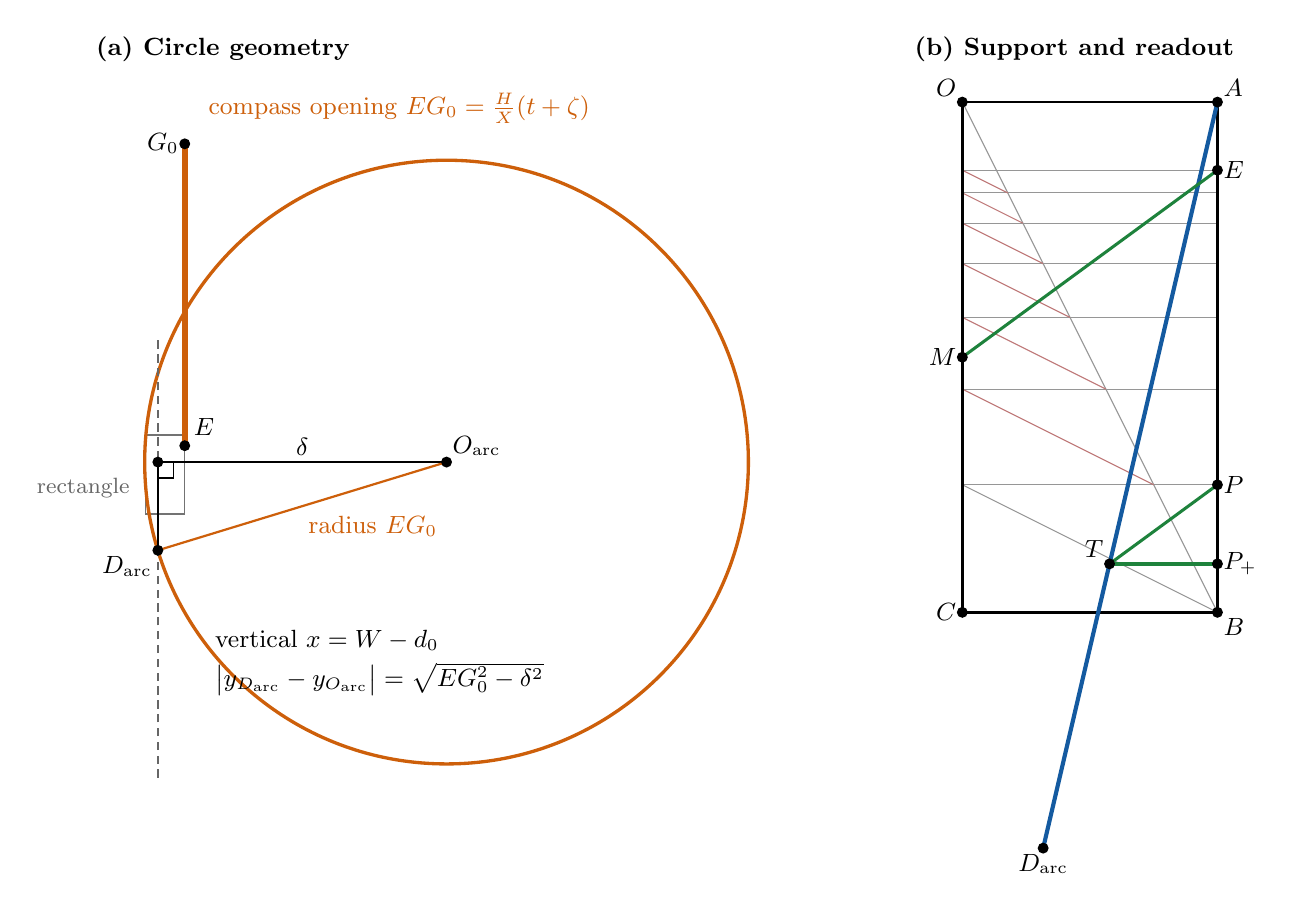
\begin{tikzpicture}[scale=0.25]
\node[ttl] at (-3,23.6) {(a) Circle geometry};
\draw[line width=0.5pt,black!55] (0,0) rectangle (2.0,4.0);
\draw[accent] (15.2980,2.6337) circle (15.3339);
\draw[aux] (0.6337,-13.4)--(0.6337,9.0);
\draw[accent,line width=2.2pt] (2.0000,3.4661)--(2.0000,18.8000);
\draw[line width=0.8pt] (0.6337,-1.8484)--(0.6337,2.6337)--(15.2980,2.6337);
\draw[line width=0.8pt,acc] (15.2980,2.6337)--(0.6337,-1.8484);
\draw[line width=0.5pt] (0.6337,1.8337)-|(1.4337,2.6337);
\node[pt] at (2.0000,18.8000) {};
\node[pt] at (2.0000,3.4661) {};
\node[pt] at (15.2980,2.6337) {};
\node[pt] at (0.6337,-1.8484) {};
\node[pt] at (0.6337,2.6337) {};
\node[lab,left] at (2.0000,18.8000) {$G_0$};
\node[lab,anchor=south west] at (2.1500,3.6661) {$E$};
\node[lab,above right] at (15.2980,2.6337) {$O_{\mathrm{arc}}$};
\node[lab,below left] at (0.6337,-1.8484) {$D_{\mathrm{arc}}$};
\node[lab,anchor=west,acc] at (2.9000,20.6) {compass opening $EG_0=\frac HX(t+\zeta)$};
\node[lab,above] at (7.9659,2.6337) {$\delta$};
\node[lab,anchor=north west,acc] at (7.9659,0.1927) {radius $EG_0$};
\node[lab,anchor=north west,align=left] at (3.2337,-5.6) {vertical $x=W-d_0$\\[3pt]$\bigl|y_{D_{\mathrm{arc}}}-y_{O_{\mathrm{arc}}}\bigr|=\sqrt{EG_0^{2}-\delta^{2}}$};
\node[font=\footnotesize,black!60,anchor=east] at (-0.3,1.3) {rectangle};
\begin{scope}[shift={(41.5,-5.0)},scale=6.48]
\node[ttl] at (-0.45,4.4136) {(b) Support and readout};
\draw[chain] (0.0000,4.0000)--(2.0000,0.0000);
\draw[chain] (0.0000,1.0000)--(2.0000,0.0000);
\draw[chain] (0,1.0000)--(2.0,1.0000);
\draw[chain] (0,1.7500)--(2.0,1.7500);
\draw[chain] (0,2.3125)--(2.0,2.3125);
\draw[chain] (0,2.7344)--(2.0,2.7344);
\draw[chain] (0,3.0508)--(2.0,3.0508);
\draw[chain] (0,3.2881)--(2.0,3.2881);
\draw[chain] (0,3.4661)--(2.0,3.4661);
\draw[chainpar] (1.5000,1.0000)--(0.0000,1.7500);
\draw[chainpar] (1.1250,1.7500)--(0.0000,2.3125);
\draw[chainpar] (0.8438,2.3125)--(0.0000,2.7344);
\draw[chainpar] (0.6328,2.7344)--(0.0000,3.0508);
\draw[chainpar] (0.4746,3.0508)--(0.0000,3.2881);
\draw[chainpar] (0.3560,3.2881)--(0.0000,3.4661);
\draw[rect] (0.0000,0.0000) rectangle (2.0000,4.0000);
\draw[support] (2.0000,4.0000)--(0.6337,-1.8484);
\draw[transport] (0.0000,2.0000)--(2.0000,3.4661);
\draw[transport] (2.0000,1.0000)--(1.1543,0.3801);
\draw[transport,line width=1.5pt] (1.1543,0.3801)--(2.0000,0.3801);
\node[lab,above left] at (0.0000,4.0000) {$O$};
\node[lab,above right] at (2.0000,4.0000) {$A$};
\node[lab,left] at (0.0000,0.0000) {$C$};
\node[lab,below right] at (2.0000,0.0000) {$B$};
\node[pt] at (0.0000,4.0000) {};
\node[pt] at (2.0000,4.0000) {};
\node[pt] at (0.0000,0.0000) {};
\node[pt] at (2.0000,0.0000) {};
\node[pt] at (0.0000,2.0000) {};
\node[pt] at (2.0000,3.4661) {};
\node[pt] at (2.0000,1.0000) {};
\node[pt] at (1.1543,0.3801) {};
\node[pt] at (2.0000,0.3801) {};
\node[lab,left] at (0.0000,2.0000) {$M$};
\node[lab,right] at (2.0000,3.4661) {$E$};
\node[lab,right] at (2.0000,1.0000) {$P$};
\node[lab,right] at (2.0000,0.3801) {$P_+$};
\node[lab,above left] at (1.1543,0.3801) {$T$};
\node[pt] at (0.6337,-1.8484) {};
\node[lab,below] at (0.6337,-1.8484) {$D_{\mathrm{arc}}$};
\end{scope}
\end{tikzpicture}%
}

\newcommand{\figMeans}{%
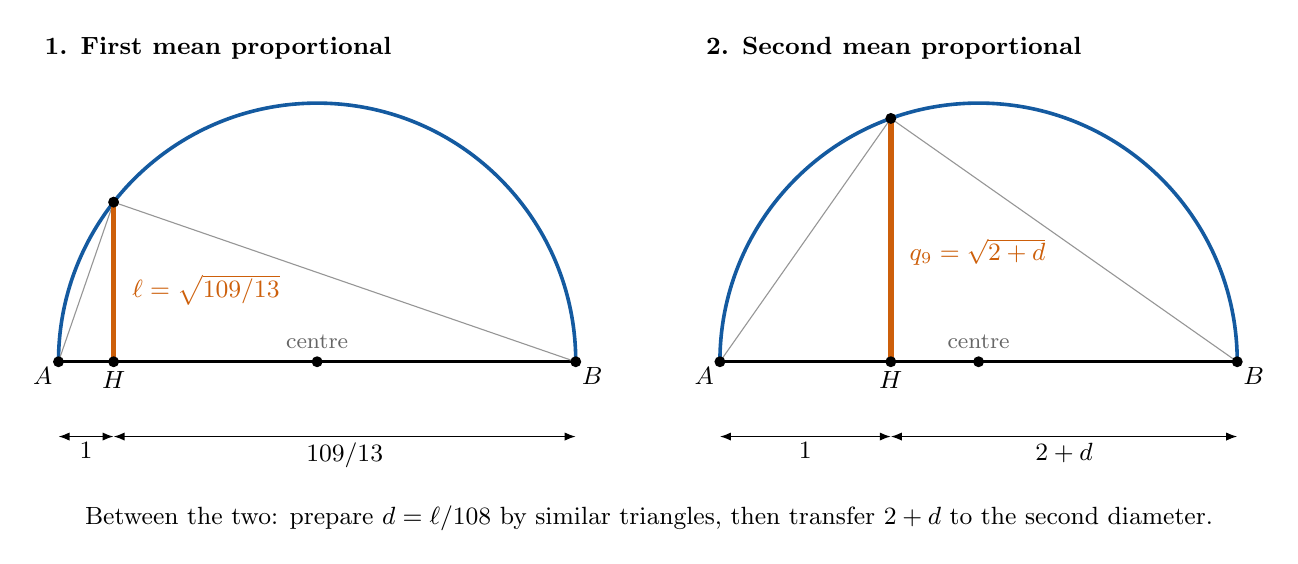
\begin{tikzpicture}
\draw[line width=1.3pt,supp] (6.5692,0) arc (0:180:3.2846);
\draw[rect] (0.0000,0)--(6.5692,0);
\draw[chain] (0.0000,0)--(0.7000,2.0269)--(6.5692,0);
\draw[accent,line width=2pt] (0.7000,0)--(0.7000,2.0269);
\node[pt] at (0.0000,0.0000) {};
\node[pt] at (0.7000,0.0000) {};
\node[pt] at (6.5692,0.0000) {};
\node[pt] at (0.7000,2.0269) {};
\node[pt] at (3.2846,0.0000) {};
\node[lab,below left] at (0.0000,0) {$A$};
\node[lab,below] at (0.7000,-0.05) {$H$};
\node[lab,below right] at (6.5692,0) {$B$};
\node[font=\footnotesize,black!60,above] at (3.2846,0.05) {centre};
\draw[dim] (0.0000,-0.95)--(0.7000,-0.95) node[midway,below,lab] {$1$};
\draw[dim] (0.7000,-0.95)--(6.5692,-0.95) node[midway,below,lab] {$109/13$};
\node[lab,acc,anchor=west,fill=white,inner sep=1.5pt] at (0.8800,0.9121) {$\ell=\sqrt{109/13}$};
\node[ttl] at (-0.3000,3.9846) {1. First mean proportional};
\draw[line width=1.3pt,supp] (14.9700,0) arc (0:180:3.2850);
\draw[rect] (8.4000,0)--(14.9700,0);
\draw[chain] (8.4000,0)--(10.5706,3.0902)--(14.9700,0);
\draw[accent,line width=2pt] (10.5706,0)--(10.5706,3.0902);
\node[pt] at (8.4000,0.0000) {};
\node[pt] at (10.5706,0.0000) {};
\node[pt] at (14.9700,0.0000) {};
\node[pt] at (10.5706,3.0902) {};
\node[pt] at (11.6850,0.0000) {};
\node[lab,below left] at (8.4000,0) {$A$};
\node[lab,below] at (10.5706,-0.05) {$H$};
\node[lab,below right] at (14.9700,0) {$B$};
\node[font=\footnotesize,black!60,above] at (11.6850,0.05) {centre};
\draw[dim] (8.4000,-0.95)--(10.5706,-0.95) node[midway,below,lab] {$1$};
\draw[dim] (10.5706,-0.95)--(14.9700,-0.95) node[midway,below,lab] {$2+d$};
\node[lab,acc,anchor=west,fill=white,inner sep=1.5pt] at (10.7506,1.3906) {$q_9=\sqrt{2+d}$};
\node[ttl] at (8.1000,3.9850) {2. Second mean proportional};
\node[lab,anchor=north,align=center] at (7.5,-1.75) {Between the two: prepare $d=\ell/108$ by similar triangles, then transfer $2+d$ to the second diameter.};
\end{tikzpicture}%
}

\newcommand{\figSupport}{%
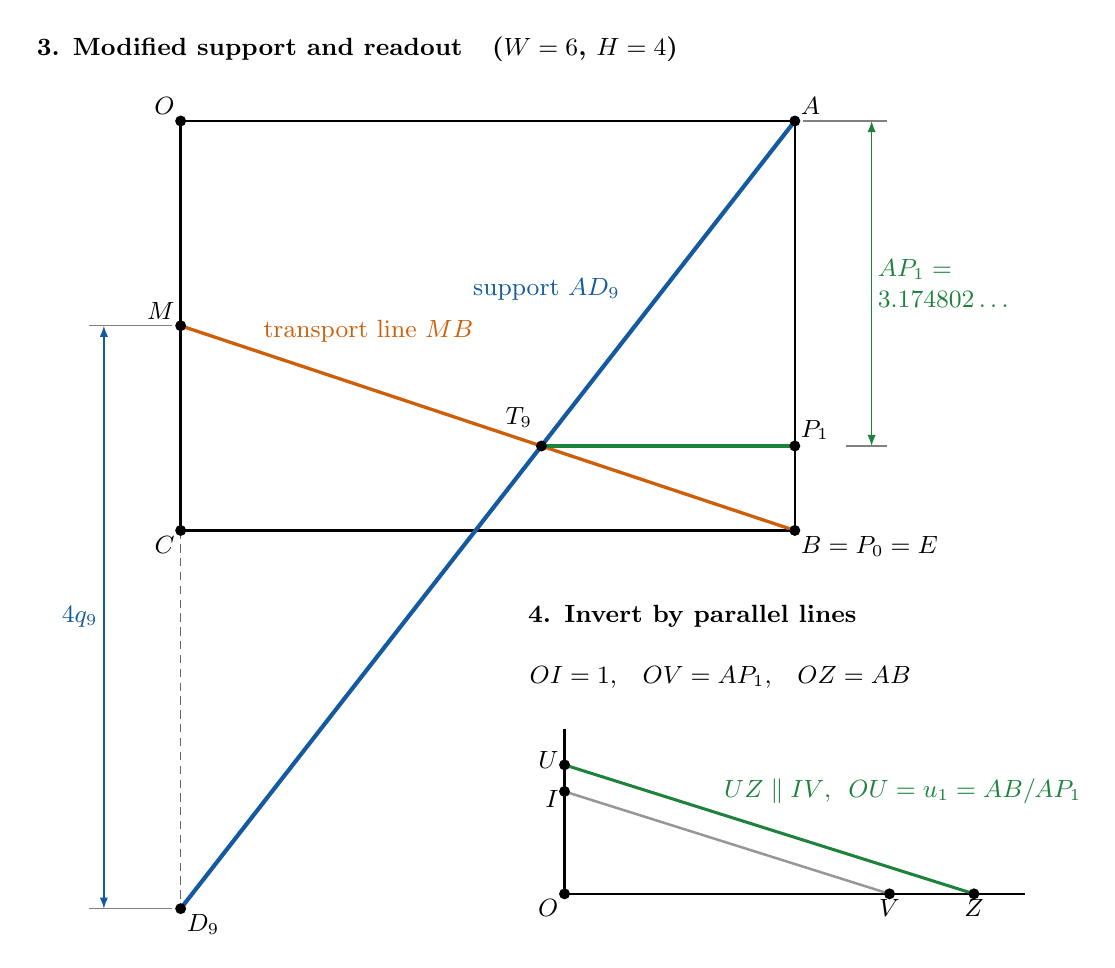
\begin{tikzpicture}[scale=1.3]
\node[ttl] at (-1.5,4.7) {3. Modified support and readout\quad($W=6$, $H=4$)};
\draw[rect] (0.0000,0.0000) rectangle (6.0000,4.0000);
\draw[aux] (0.0000,0.0000)--(0.0000,-3.6946);
\draw[accent] (0.0000,2.0000)--(6.0000,0.0000);
\draw[support] (6.0000,4.0000)--(0.0000,-3.6946);
\draw[transport,line width=1.6pt] (3.5244,0.8252)--(6.0000,0.8252);
\node[pt] at (0.0000,4.0000) {};
\node[pt] at (6.0000,4.0000) {};
\node[pt] at (0.0000,0.0000) {};
\node[pt] at (6.0000,0.0000) {};
\node[pt] at (0.0000,2.0000) {};
\node[pt] at (0.0000,-3.6946) {};
\node[pt] at (3.5244,0.8252) {};
\node[pt] at (6.0000,0.8252) {};
\node[lab,above left] at (0.0000,4.0000) {$O$};
\node[lab,above right] at (6.0000,4.0000) {$A$};
\node[lab,below left] at (0.0000,0.0000) {$C$};
\node[lab,below right] at (6.0000,0.0000) {$B=P_0=E$};
\node[lab,above left] at (0.0000,2.0000) {$M$};
\node[lab,below right] at (0.0000,-3.6946) {$D_9$};
\node[lab,anchor=south] at (3.3044,0.9452) {$T_9$};
\node[lab,above right] at (6.0000,0.8252) {$P_1$};
\draw[dim,supp] (-0.75,2.0000)--(-0.75,-3.6946) node[midway,left,lab,supp] {$4q_9$};
\draw[line width=0.4pt,black!50] (-0.9,2.0000)--(-0.08,2.0000) (-0.9,-3.6946)--(-0.08,-3.6946);
\draw[dim,trans] (6.75,4.0000)--(6.75,0.8252) node[midway,right,lab,trans,align=left] {$AP_1=$\\$3.174802\ldots$};
\draw[line width=0.4pt,black!50] (6.08,4.0000)--(6.9,4.0000) (6.5,0.8252)--(6.9,0.8252);
\node[lab,supp,anchor=east] at (4.35,2.35) {support $AD_9$};
\node[lab,acc,anchor=south west] at (0.75,1.78) {transport line $MB$};
\begin{scope}[shift={(3.75,-3.55)}]
\node[ttl] at (-0.45,2.7099) {4. Invert by parallel lines};
\node[lab,anchor=west] at (-0.4,2.1099) {$OI=1$,\quad $OV=AP_1$,\quad $OZ=AB$};
\draw[rect] (0,0)--(4.5,0) (0,0)--(0,1.6099);
\draw[chain,line width=0.9pt] (0,1)--(3.1748,0);
\draw[transport] (0,1.2599)--(4,0);
\node[pt] at (0.0000,0.0000) {};
\node[pt] at (0.0000,1.0000) {};
\node[pt] at (0.0000,1.2599) {};
\node[pt] at (3.1748,0.0000) {};
\node[pt] at (4.0000,0.0000) {};
\node[lab,below left] at (0,0) {$O$};
\node[lab,left] at (0,0.93) {$I$};
\node[lab,left] at (0,1.3099) {$U$};
\node[lab,below] at (3.1748,0) {$V$};
\node[lab,below] at (4,0) {$Z$};
\node[lab,anchor=south west,trans] at (1.5,0.82) {$UZ\parallel IV$,\ \ $OU=u_1=AB/AP_1$};
\end{scope}
\end{tikzpicture}%
}

\newcommand{\figSubdivision}{%
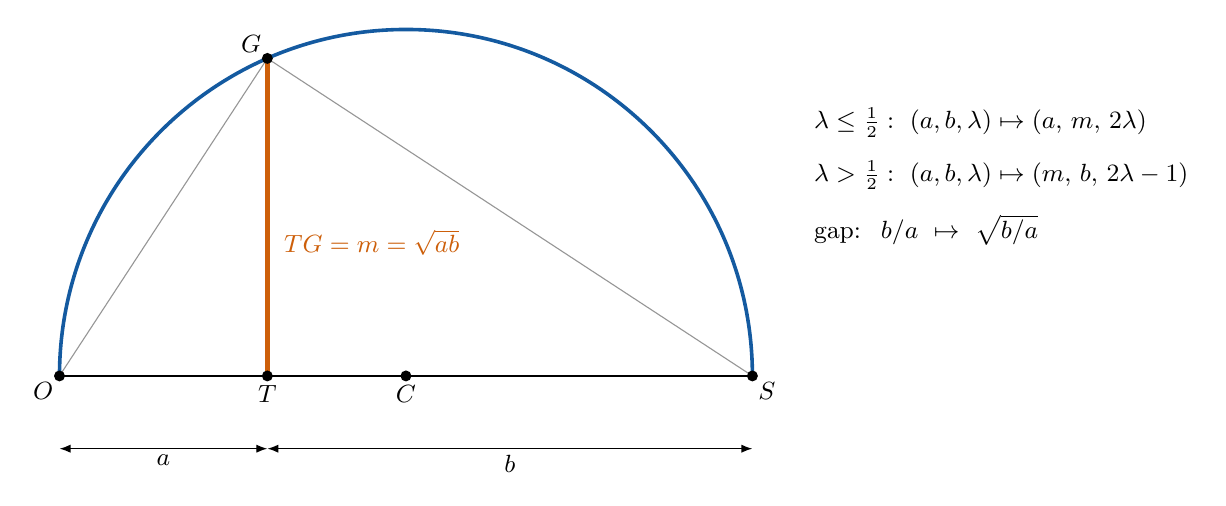
\begin{tikzpicture}[scale=2.2]
\draw[line width=1.3pt,supp] (4.0,0) arc (0:180:2.0);
\draw[rect] (0,0)--(4.0,0);
\draw[chain] (0,0)--(1.2,1.8330)--(4.0,0);
\draw[accent,line width=2pt] (1.2,0)--(1.2,1.8330);
\node[pt] at (0.0000,0.0000) {};
\node[pt] at (1.2000,0.0000) {};
\node[pt] at (2.0000,0.0000) {};
\node[pt] at (4.0000,0.0000) {};
\node[pt] at (1.2000,1.8330) {};
\node[lab,below left] at (0,0) {$O$};
\node[lab,below] at (1.2,-0.02) {$T$};
\node[lab,below] at (2.0,-0.02) {$C$};
\node[lab,below right] at (4.0,0) {$S$};
\node[lab,above left] at (1.2,1.8330) {$G$};
\node[lab,acc,anchor=west,fill=white,inner sep=1.5pt] at (1.27,0.7699) {$TG=m=\sqrt{ab}$};
\draw[dim] (0,-0.42)--(1.2,-0.42) node[midway,below,lab] {$a$};
\draw[dim] (1.2,-0.42)--(4.0,-0.42) node[midway,below,lab] {$b$};
\node[anchor=west,align=left,font=\small] at (4.3,1.15) {$\lambda\le\tfrac12:\ (a,b,\lambda)\mapsto(a,\,m,\,2\lambda)$\\[8pt]$\lambda>\tfrac12:\ (a,b,\lambda)\mapsto(m,\,b,\,2\lambda-1)$\\[8pt]gap: $\ b/a\ \mapsto\ \sqrt{b/a}$};
\end{tikzpicture}%
}

\newcommand{\figDepth}{%
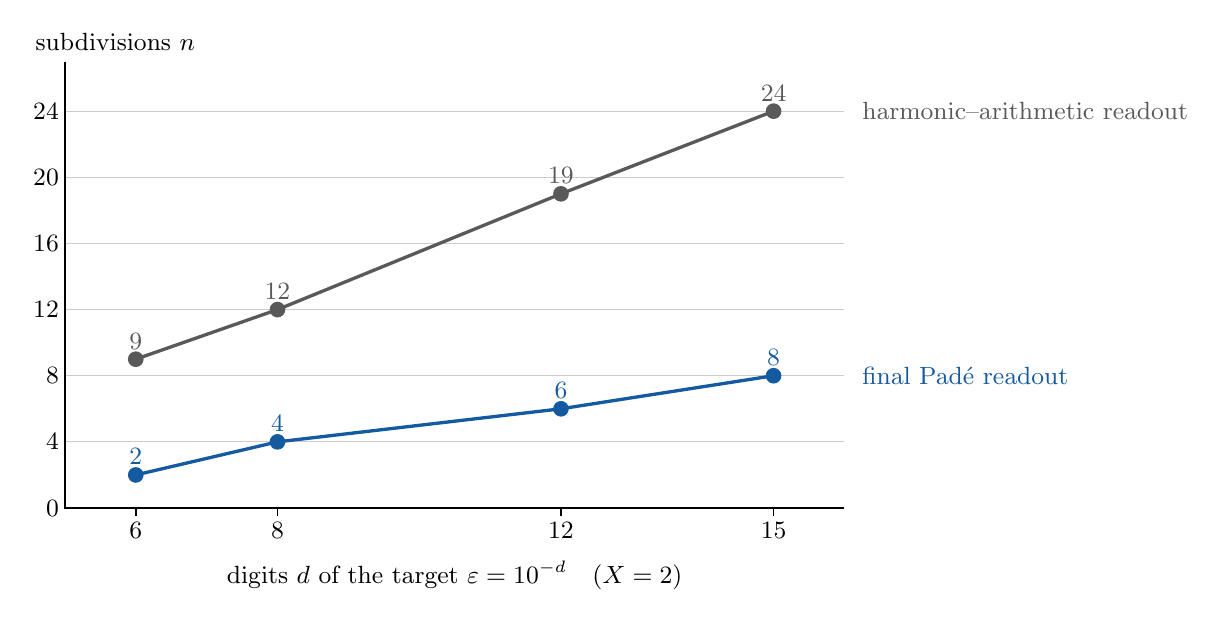
\begin{tikzpicture}
\draw[line width=0.3pt,black!20] (0,0.000)--(9.900,0.000);
\node[lab,left] at (0,0.000) {0};
\draw[line width=0.3pt,black!20] (0,0.840)--(9.900,0.840);
\node[lab,left] at (0,0.840) {4};
\draw[line width=0.3pt,black!20] (0,1.680)--(9.900,1.680);
\node[lab,left] at (0,1.680) {8};
\draw[line width=0.3pt,black!20] (0,2.520)--(9.900,2.520);
\node[lab,left] at (0,2.520) {12};
\draw[line width=0.3pt,black!20] (0,3.360)--(9.900,3.360);
\node[lab,left] at (0,3.360) {16};
\draw[line width=0.3pt,black!20] (0,4.200)--(9.900,4.200);
\node[lab,left] at (0,4.200) {20};
\draw[line width=0.3pt,black!20] (0,5.040)--(9.900,5.040);
\node[lab,left] at (0,5.040) {24};
\draw[rect] (0,5.670)--(0,0)--(9.900,0);
\draw[line width=0.6pt] (0.900,0)--(0.900,-0.1);
\node[lab,below] at (0.900,-0.1) {6};
\draw[line width=0.6pt] (2.700,0)--(2.700,-0.1);
\node[lab,below] at (2.700,-0.1) {8};
\draw[line width=0.6pt] (6.300,0)--(6.300,-0.1);
\node[lab,below] at (6.300,-0.1) {12};
\draw[line width=0.6pt] (9.000,0)--(9.000,-0.1);
\node[lab,below] at (9.000,-0.1) {15};
\draw[line width=1.2pt,black!65] (0.900,1.890)--(2.700,2.520)--(6.300,3.990)--(9.000,5.040);
\node[circle,fill=black!65,inner sep=2pt] at (0.900,1.890) {};
\node[lab,above,black!65] at (0.900,1.940) {9};
\node[circle,fill=black!65,inner sep=2pt] at (2.700,2.520) {};
\node[lab,above,black!65] at (2.700,2.570) {12};
\node[circle,fill=black!65,inner sep=2pt] at (6.300,3.990) {};
\node[lab,above,black!65] at (6.300,4.040) {19};
\node[circle,fill=black!65,inner sep=2pt] at (9.000,5.040) {};
\node[lab,above,black!65] at (9.000,5.090) {24};
\node[lab,black!65,anchor=west] at (10.050,5.040) {harmonic--arithmetic readout};
\draw[line width=1.2pt,supp] (0.900,0.420)--(2.700,0.840)--(6.300,1.260)--(9.000,1.680);
\node[circle,fill=supp,inner sep=2pt] at (0.900,0.420) {};
\node[lab,above,supp] at (0.900,0.470) {2};
\node[circle,fill=supp,inner sep=2pt] at (2.700,0.840) {};
\node[lab,above,supp] at (2.700,0.890) {4};
\node[circle,fill=supp,inner sep=2pt] at (6.300,1.260) {};
\node[lab,above,supp] at (6.300,1.310) {6};
\node[circle,fill=supp,inner sep=2pt] at (9.000,1.680) {};
\node[lab,above,supp] at (9.000,1.730) {8};
\node[lab,supp,anchor=west] at (10.050,1.680) {final Pad\'e readout};
\node[lab,anchor=south west] at (-0.45,5.733) {subdivisions $n$};
\node[lab,anchor=north] at (4.950,-0.6) {digits $d$ of the target $\varepsilon=10^{-d}$\quad($X=2$)};
\end{tikzpicture}%
}

\newcommand{\figAK}{%
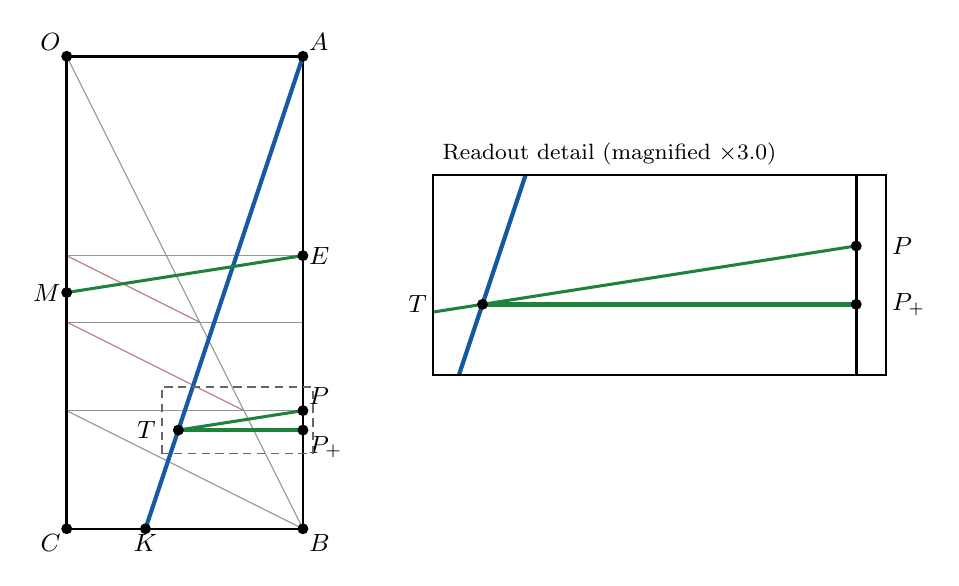
\begin{tikzpicture}[scale=1.5]
\draw[chain] (0.0000,4.0000)--(2.0000,0.0000);
\draw[chain] (0.0000,1.0000)--(2.0000,0.0000);
\draw[chain] (0,1.0000)--(2.0,1.0000);
\draw[chain] (0,1.7500)--(2.0,1.7500);
\draw[chain] (0,2.3125)--(2.0,2.3125);
\draw[chainpar] (1.5000,1.0000)--(0.0000,1.7500);
\draw[chainpar] (1.1250,1.7500)--(0.0000,2.3125);
\draw[rect] (0.0000,0.0000) rectangle (2.0000,4.0000);
\draw[support] (2.0000,4.0000)--(0.6667,0.0000);
\draw[transport] (0.0000,2.0000)--(2.0000,2.3125);
\draw[transport] (2.0000,1.0000)--(0.9451,0.8352);
\draw[transport,line width=1.5pt] (0.9451,0.8352)--(2.0000,0.8352);
\node[lab,above left] at (0.0000,4.0000) {$O$};
\node[lab,above right] at (2.0000,4.0000) {$A$};
\node[lab,below left] at (0.0000,0.0000) {$C$};
\node[lab,below right] at (2.0000,0.0000) {$B$};
\node[pt] at (0.0000,4.0000) {};
\node[pt] at (2.0000,4.0000) {};
\node[pt] at (0.0000,0.0000) {};
\node[pt] at (2.0000,0.0000) {};
\node[pt] at (0.0000,2.0000) {};
\node[pt] at (2.0000,2.3125) {};
\node[pt] at (2.0000,1.0000) {};
\node[pt] at (0.9451,0.8352) {};
\node[pt] at (2.0000,0.8352) {};
\node[lab,left] at (0.0000,2.0000) {$M$};
\node[lab,right] at (2.0000,2.3125) {$E$};
\node[lab,above right] at (2.0000,1.0000) {$P$};
\node[lab,below right] at (2.0000,0.8352) {$P_+$};
\node[pt] at (0.6667,0.0000) {};
\node[lab,below] at (0.6667,0.0000) {$K$};
\draw[aux] (0.8051,0.6352) rectangle (2.0840,1.2000);
\node[lab,left] at (0.8051,0.8352) {$T$};
\begin{scope}[shift={(0.6848,-0.6055)},scale=3.0]
\begin{scope}
\clip (0.8051,0.6352) rectangle (2.0840,1.2000);
\fill[white] (0.8051,0.6352) rectangle (2.0840,1.2000);
\draw[rect] (2.0,-0.3648)--(2.0,2.2000);
\draw[support] (2.0000,4.0000)--(0.6667,0.0000);
\draw[transport] (2.0000,1.0000)--(-3.0000,0.2188);
\draw[transport,line width=1.6pt] (0.9451,0.8352)--(2.0000,0.8352);
\node[pt] at (2.0000,1.0000) {};
\node[pt] at (0.9451,0.8352) {};
\node[pt] at (2.0000,0.8352) {};
\end{scope}
\draw[line width=0.6pt] (0.8051,0.6352) rectangle (2.0840,1.2000);
\node[lab,right] at (2.0840,1.0000) {$P$};
\node[lab,right] at (2.0840,0.8352) {$P_+$};
\node[lab,left] at (0.8051,0.8352) {$T$};
\node[font=\footnotesize,anchor=south west] at (0.8051,1.2000) {Readout detail (magnified $\times3.0$)};
\end{scope}
\end{tikzpicture}%
}

\newcommand{\figAD}{%
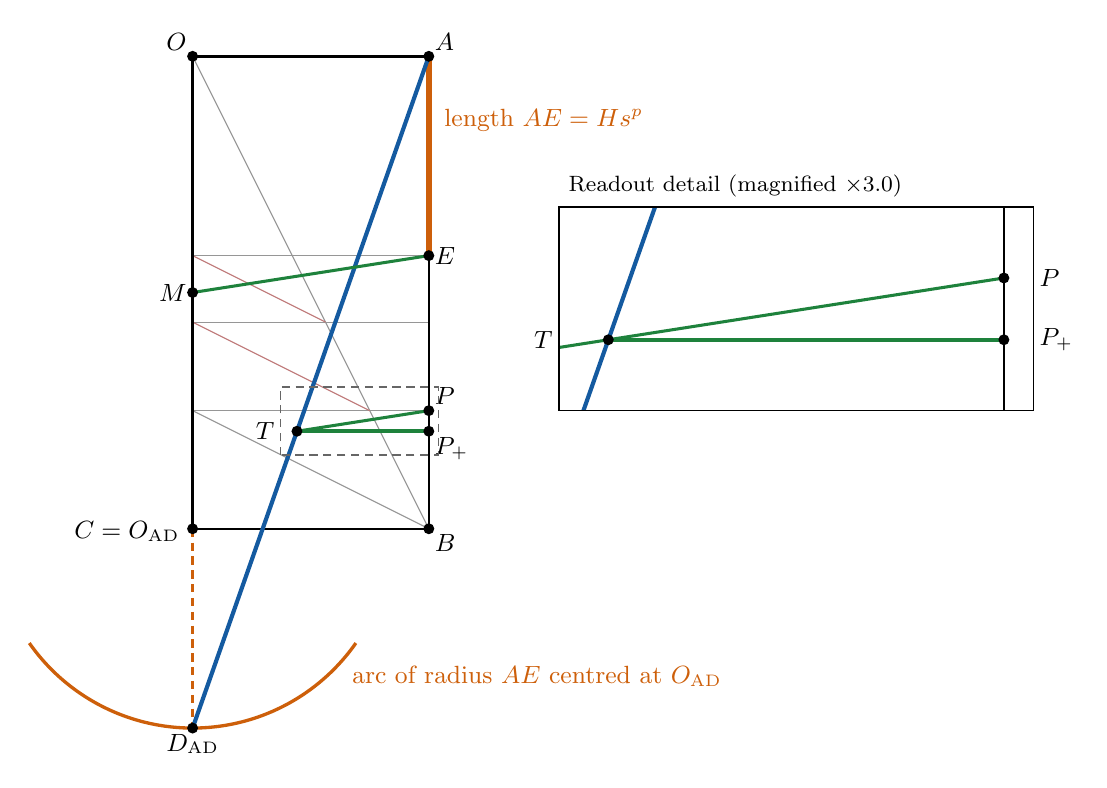
\begin{tikzpicture}[scale=1.5]
\draw[chain] (0.0000,4.0000)--(2.0000,0.0000);
\draw[chain] (0.0000,1.0000)--(2.0000,0.0000);
\draw[chain] (0,1.0000)--(2.0,1.0000);
\draw[chain] (0,1.7500)--(2.0,1.7500);
\draw[chain] (0,2.3125)--(2.0,2.3125);
\draw[chainpar] (1.5000,1.0000)--(0.0000,1.7500);
\draw[chainpar] (1.1250,1.7500)--(0.0000,2.3125);
\draw[rect] (0.0000,0.0000) rectangle (2.0000,4.0000);
\draw[accent] (0.0000,0.0000) ++(215:1.6875) arc (215:325:1.6875);
\draw[accent,densely dashed] (0.0000,0.0000)--(0.0000,-1.6875);
\draw[accent,line width=2.2pt] (2.0000,4.0000)--(2.0000,2.3125);
\draw[support] (2.0000,4.0000)--(0.0000,-1.6875);
\draw[transport] (0.0000,2.0000)--(2.0000,2.3125);
\draw[transport] (2.0000,1.0000)--(0.8837,0.8256);
\draw[transport,line width=1.5pt] (0.8837,0.8256)--(2.0000,0.8256);
\node[lab,above left] at (0.0000,4.0000) {$O$};
\node[lab,above right] at (2.0000,4.0000) {$A$};
\node[lab,anchor=east] at (-0.06,-0.02) {$C=O_{\mathrm{AD}}$};
\node[lab,below right] at (2.0000,0.0000) {$B$};
\node[pt] at (0.0000,4.0000) {};
\node[pt] at (2.0000,4.0000) {};
\node[pt] at (0.0000,0.0000) {};
\node[pt] at (2.0000,0.0000) {};
\node[pt] at (0.0000,2.0000) {};
\node[pt] at (2.0000,2.3125) {};
\node[pt] at (2.0000,1.0000) {};
\node[pt] at (0.8837,0.8256) {};
\node[pt] at (2.0000,0.8256) {};
\node[lab,left] at (0.0000,2.0000) {$M$};
\node[lab,right] at (2.0000,2.3125) {$E$};
\node[lab,above right] at (2.0000,1.0000) {$P$};
\node[lab,below right] at (2.0000,0.8256) {$P_+$};
\node[pt] at (0.0000,-1.6875) {};
\node[lab,below] at (0.0000,-1.6875) {$D_{\mathrm{AD}}$};
\node[lab,acc,anchor=west] at (2.0800,3.4562) {length $AE=Hs^p$};
\node[lab,acc,anchor=west] at (1.3,-1.25) {arc of radius $AE$ centred at $O_{\mathrm{AD}}$};
\draw[aux] (0.7437,0.6256) rectangle (2.0840,1.2000);
\node[lab,left] at (0.7437,0.8256) {$T$};
\begin{scope}[shift={(0.8688,-0.8767)},scale=3.0]
\begin{scope}
\clip (0.7437,0.6256) rectangle (2.0840,1.2000);
\fill[white] (0.7437,0.6256) rectangle (2.0840,1.2000);
\draw[rect] (2.0,-0.3744)--(2.0,2.2000);
\draw[support] (2.0000,4.0000)--(0.0000,-1.6875);
\draw[transport] (2.0000,1.0000)--(-3.0000,0.2188);
\draw[transport,line width=1.6pt] (0.8837,0.8256)--(2.0000,0.8256);
\node[pt] at (2.0000,1.0000) {};
\node[pt] at (0.8837,0.8256) {};
\node[pt] at (2.0000,0.8256) {};
\end{scope}
\draw[line width=0.6pt] (0.7437,0.6256) rectangle (2.0840,1.2000);
\node[lab,right] at (2.0840,1.0000) {$P$};
\node[lab,right] at (2.0840,0.8256) {$P_+$};
\node[lab,left] at (0.7437,0.8256) {$T$};
\node[font=\footnotesize,anchor=south west] at (0.7437,1.2000) {Readout detail (magnified $\times3.0$)};
\end{scope}
\end{tikzpicture}%
}

\newcommand{\figProjective}{%
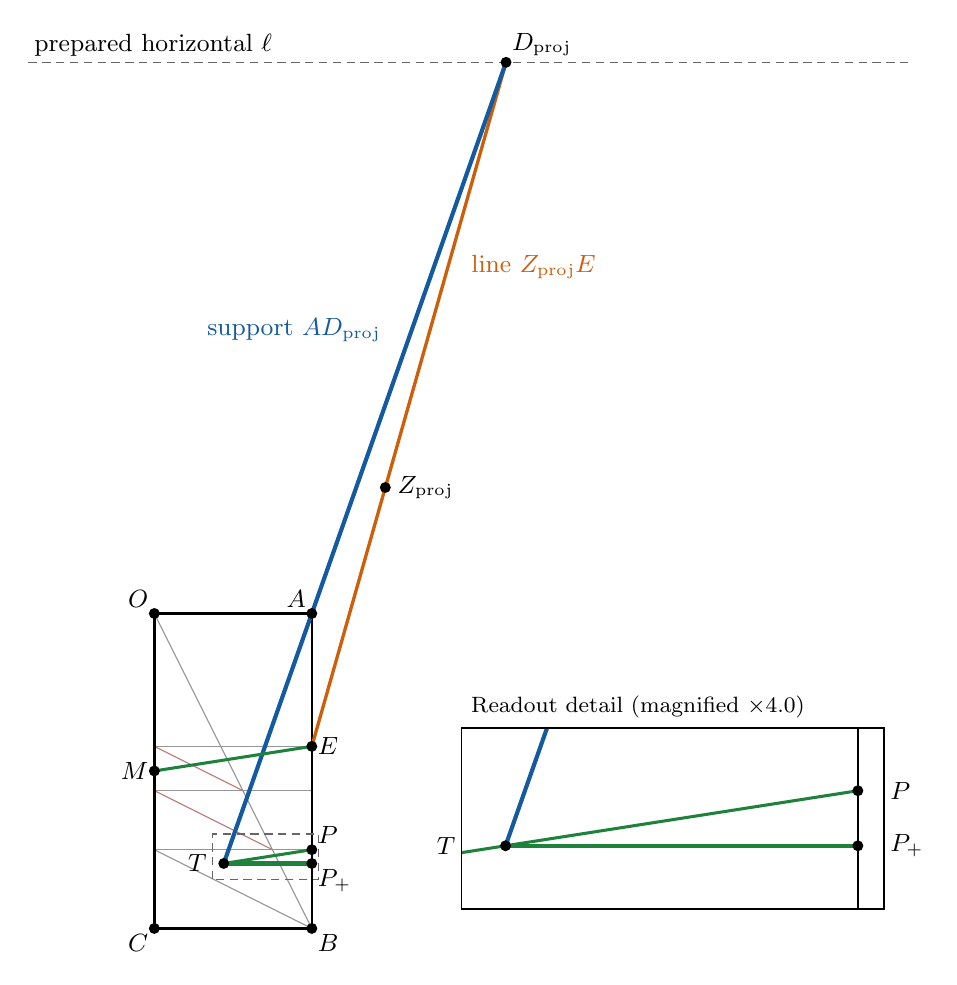
\begin{tikzpicture}[scale=1.0]
\draw[aux] (-1.6,11.0000)--(9.6,11.0000);
\node[lab,anchor=south west] at (-1.6,11.0000) {prepared horizontal $\ell$};
\draw[chain] (0.0000,4.0000)--(2.0000,0.0000);
\draw[chain] (0.0000,1.0000)--(2.0000,0.0000);
\draw[chain] (0,1.0000)--(2.0,1.0000);
\draw[chain] (0,1.7500)--(2.0,1.7500);
\draw[chain] (0,2.3125)--(2.0,2.3125);
\draw[chainpar] (1.5000,1.0000)--(0.0000,1.7500);
\draw[chainpar] (1.1250,1.7500)--(0.0000,2.3125);
\draw[rect] (0.0000,0.0000) rectangle (2.0000,4.0000);
\draw[accent] (2.0000,2.3125)--(4.4664,11.0000);
\draw[support] (0.8814,0.8252)--(4.4664,11.0000);
\draw[transport] (0.0000,2.0000)--(2.0000,2.3125);
\draw[transport] (2.0000,1.0000)--(0.8814,0.8252);
\draw[transport,line width=1.5pt] (0.8814,0.8252)--(2.0000,0.8252);
\node[lab,above left] at (0.0000,4.0000) {$O$};
\node[lab,above left] at (2.0000,4.0000) {$A$};
\node[lab,below left] at (0.0000,0.0000) {$C$};
\node[lab,below right] at (2.0000,0.0000) {$B$};
\node[pt] at (0.0000,4.0000) {};
\node[pt] at (2.0000,4.0000) {};
\node[pt] at (0.0000,0.0000) {};
\node[pt] at (2.0000,0.0000) {};
\node[pt] at (0.0000,2.0000) {};
\node[pt] at (2.0000,2.3125) {};
\node[pt] at (2.0000,1.0000) {};
\node[pt] at (0.8814,0.8252) {};
\node[pt] at (2.0000,0.8252) {};
\node[lab,left] at (0.0000,2.0000) {$M$};
\node[lab,right] at (2.0000,2.3125) {$E$};
\node[lab,above right] at (2.0000,1.0000) {$P$};
\node[lab,below right] at (2.0000,0.8252) {$P_+$};
\node[pt] at (2.9333,5.6000) {};
\node[pt] at (4.4664,11.0000) {};
\node[lab,right] at (3.0133,5.6000) {$Z_{\mathrm{proj}}$};
\node[lab,above right] at (4.4664,11.0000) {$D_{\mathrm{proj}}$};
\node[lab,acc,anchor=west] at (3.95,8.4) {line $Z_{\mathrm{proj}}E$};
\node[lab,supp,anchor=east] at (2.95,7.6) {support $AD_{\mathrm{proj}}$};
\draw[aux] (0.7414,0.6252) rectangle (2.0840,1.2000);
\node[lab,left] at (0.7414,0.8252) {$T$};
\begin{scope}[shift={(0.9345,-2.2509)},scale=4.0]
\begin{scope}
\clip (0.7414,0.6252) rectangle (2.0840,1.2000);
\fill[white] (0.7414,0.6252) rectangle (2.0840,1.2000);
\draw[rect] (2.0,-0.3748)--(2.0,2.2000);
\draw[support] (0.8814,0.8252)--(4.4664,11.0000);
\draw[transport] (2.0000,1.0000)--(-3.0000,0.2188);
\draw[transport,line width=1.6pt] (0.8814,0.8252)--(2.0000,0.8252);
\node[pt] at (2.0000,1.0000) {};
\node[pt] at (0.8814,0.8252) {};
\node[pt] at (2.0000,0.8252) {};
\end{scope}
\draw[line width=0.6pt] (0.7414,0.6252) rectangle (2.0840,1.2000);
\node[lab,right] at (2.0840,1.0000) {$P$};
\node[lab,right] at (2.0840,0.8252) {$P_+$};
\node[lab,left] at (0.7414,0.8252) {$T$};
\node[font=\footnotesize,anchor=south west] at (0.7414,1.2000) {Readout detail (magnified $\times4.0$)};
\end{scope}
\end{tikzpicture}%
}

\newcommand{\figMA}{%
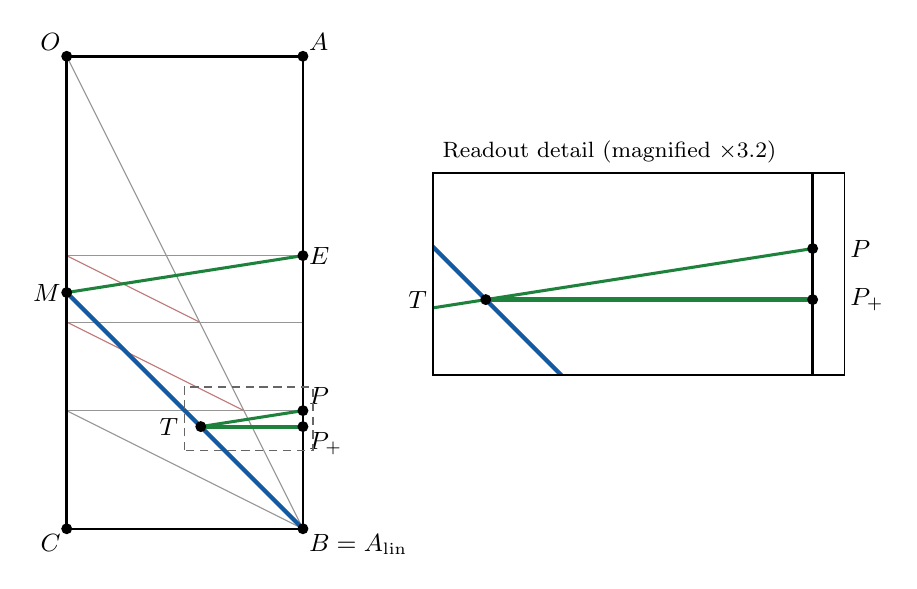
\begin{tikzpicture}[scale=1.5]
\draw[chain] (0.0000,4.0000)--(2.0000,0.0000);
\draw[chain] (0.0000,1.0000)--(2.0000,0.0000);
\draw[chain] (0,1.0000)--(2.0,1.0000);
\draw[chain] (0,1.7500)--(2.0,1.7500);
\draw[chain] (0,2.3125)--(2.0,2.3125);
\draw[chainpar] (1.5000,1.0000)--(0.0000,1.7500);
\draw[chainpar] (1.1250,1.7500)--(0.0000,2.3125);
\draw[rect] (0.0000,0.0000) rectangle (2.0000,4.0000);
\draw[support] (0.0000,2.0000)--(2.0000,0.0000);
\draw[transport] (0.0000,2.0000)--(2.0000,2.3125);
\draw[transport] (2.0000,1.0000)--(1.1351,0.8649);
\draw[transport,line width=1.5pt] (1.1351,0.8649)--(2.0000,0.8649);
\node[lab,above left] at (0.0000,4.0000) {$O$};
\node[lab,above right] at (2.0000,4.0000) {$A$};
\node[lab,below left] at (0.0000,0.0000) {$C$};
\node[lab,below right] at (2.0000,0.0000) {$B=A_{\mathrm{lin}}$};
\node[pt] at (0.0000,4.0000) {};
\node[pt] at (2.0000,4.0000) {};
\node[pt] at (0.0000,0.0000) {};
\node[pt] at (2.0000,0.0000) {};
\node[pt] at (0.0000,2.0000) {};
\node[pt] at (2.0000,2.3125) {};
\node[pt] at (2.0000,1.0000) {};
\node[pt] at (1.1351,0.8649) {};
\node[pt] at (2.0000,0.8649) {};
\node[lab,left] at (0.0000,2.0000) {$M$};
\node[lab,right] at (2.0000,2.3125) {$E$};
\node[lab,above right] at (2.0000,1.0000) {$P$};
\node[lab,below right] at (2.0000,0.8649) {$P_+$};
\draw[aux] (0.9951,0.6649) rectangle (2.0840,1.2000);
\node[lab,left] at (0.9951,0.8649) {$T$};
\begin{scope}[shift={(-0.0844,-0.8276)},scale=3.2]
\begin{scope}
\clip (0.9951,0.6649) rectangle (2.0840,1.2000);
\fill[white] (0.9951,0.6649) rectangle (2.0840,1.2000);
\draw[rect] (2.0,-0.3351)--(2.0,2.2000);
\draw[support] (0.0000,2.0000)--(2.0000,0.0000);
\draw[transport] (2.0000,1.0000)--(-3.0000,0.2188);
\draw[transport,line width=1.6pt] (1.1351,0.8649)--(2.0000,0.8649);
\node[pt] at (2.0000,1.0000) {};
\node[pt] at (1.1351,0.8649) {};
\node[pt] at (2.0000,0.8649) {};
\end{scope}
\draw[line width=0.6pt] (0.9951,0.6649) rectangle (2.0840,1.2000);
\node[lab,right] at (2.0840,1.0000) {$P$};
\node[lab,right] at (2.0840,0.8649) {$P_+$};
\node[lab,left] at (0.9951,0.8649) {$T$};
\node[font=\footnotesize,anchor=south west] at (0.9951,1.2000) {Readout detail (magnified $\times3.2$)};
\end{scope}
\end{tikzpicture}%
}



\pagestyle{fancy}\fancyhf{}
\fancyhead[L]{\small Geometric root calculators}
\fancyhead[R]{\small V28 / Research preprint}
\fancyfoot[C]{\small\thepage}
\renewcommand{\headrulewidth}{0.3pt}
\setlength{\parindent}{0pt}\setlength{\parskip}{5pt plus 1pt}
\setlist{itemsep=2pt,topsep=3pt}

\theoremstyle{plain}
\newtheorem{theorem}{Theorem}[section]
\newtheorem{proposition}[theorem]{Proposition}
\newtheorem{lemma}[theorem]{Lemma}
\newtheorem{corollary}[theorem]{Corollary}
\theoremstyle{remark}
\newtheorem{remark}[theorem]{Remark}
\numberwithin{equation}{section}

% ---- notation macros ---------------------------------------------------
\newcommand{\jn}{\mathsf{j}}          % one join
\newcommand{\pl}{\mathsf{p}}          % one constructed parallel (= 2j + 3c)
\newcommand{\ar}{\mathsf{c}}          % one compass arc
\newcommand{\Om}{\Omega}              % projection centres on the top line
\newcommand{\cE}{\mathcal{E}}\newcommand{\cC}{\mathcal{C}}\newcommand{\cD}{\mathcal{D}}
\newcommand{\cU}{\mathcal{U}}\newcommand{\cV}{\mathcal{V}}\newcommand{\cR}{\mathcal{R}}
\newcommand{\cJ}{\mathcal{J}}\newcommand{\cA}{\mathcal{A}}\newcommand{\cB}{\mathcal{B}}
\newcommand{\cK}{\mathcal{K}}\newcommand{\cM}{\mathcal{M}}\newcommand{\cP}{\mathcal{P}}
\newcommand{\Tm}{\mathrm{T}}
\newcommand{\eps}{\varepsilon}
\DeclareMathOperator{\disc}{disc}

\begin{document}

{\small\scshape Constructive geometry \,/\, root iterations \,/\, global convergence}

\vspace{6pt}
{\LARGE\bfseries Geometric Root Calculators\par}
\vspace{3pt}
{\large A ninth-order nested-radical support and real-degree enclosures in the Pandrosion rectangle\par}
\vspace{8pt}
Ivan Besevic\footnote{Computational assistance: AI was used for derivations, proof development,
figures and manuscript preparation. The author is responsible for the claims and their attribution.
Section~\ref{sec:evidence} states, claim by claim, which results are formal proofs, written proofs,
computer-algebra identities or numerical checks.}
\quad$\cdot$\quad Independent research\\
Version 28 (revision of V27-NR) \quad$\cdot$\quad 12 November 2026\\
\url{https://github.com/ivan-fr/pandrosion}

\vspace{6pt}
\begin{quote}\small
\textbf{Abstract.}
We study ruler-and-compass iterations for the positive root $X^{1/p}$ that share one rectangle, one
power stage and one readout, and differ only in a \emph{support line}. Every support approximates the
same target function $\kappa_*(t)=(t-1)/(t^{1/p}-1)$ of the residual $t$, and the contact order of the
approximation fixes the order of the iteration. Besides the classical supports of orders one to four we
treat two radical supports. A decentered arc gives a globally monotone fifth-order iteration. A support
built from two successive mean proportionals has local order \emph{exactly nine for every real $p>2$},
with an explicit positive error constant equal to $7/648$ for cube roots, and converges monotonically
from every positive start. For integer $p\ge 3$ one nested-radical step costs at most $10p+59$
elementary traces against $10p+9$ for the decentered arc; measured by the efficiency index the
decentered arc is preferable for $p\le 12$ and the nested support for $p\ge 13$. We then separate what
is a finite construction from what is only a scalar statement: the fast iterations are finite
constructions for rational degrees, whereas for irrational $p$ a single step is not. For arbitrary real
$p\neq 0$ a power-free subdivision with one final Pad\'e readout encloses the root with relative width at
most $z^5/256$ in at most $15n+63$ traces after $n$ subdivisions (for $X>1$, $p\ge 1$). Global
convergence and the local orders with their constants, for both radical supports and every real
$p>2$, are checked in Lean, as are the degree, approximation and efficiency statements; the drawing
inventories are written protocols.
\end{quote}

% =========================================================================
\section{Introduction}

A geometric iteration must realize its arithmetic by intersections, parallels and length transfers.
The Pandrosion rectangle does this for $p$th roots: a chain of similar triangles produces the power
$s^p$ of the current estimate, a line through a prepared point transports the residual, and a horizontal
reads the next estimate on the same rail. The only part that changes from one method to another is the
\emph{support}, a line through the corner $A$ whose slope encodes a correction factor.

\paragraph{Results.}
\begin{enumerate}[label=\arabic*.]
\item \textbf{One target function} (Section~\ref{sec:coords}). All supports approximate
  $\kappa_*(t)=(t-1)/(t^{1/p}-1)$; contact of order $\omega$ at $t=1$ gives an iteration of order $\omega+1$ with
  an explicit error constant (Lemma~\ref{lem:contact}). Newton, Halley and the $[1/1]$ Pad\'e support are
  the cases $\omega=1,2,3$.
\item \textbf{Decentered arc} (Section~\ref{sec:arc}). One moving arc and one join give $\omega=4$:
  a fifth-order iteration, monotone and convergent from every positive start for real $p>2$
  (Theorem~\ref{thm:arc}).
\item \textbf{Nested radicals} (Section~\ref{sec:nested}). Two successive mean proportionals give
  $\omega=8$. The iteration has order exactly nine for every real $p>2$, with the closed-form constant of
  Theorem~\ref{thm:order9}; it is globally monotone (Theorem~\ref{thm:global}).
\item \textbf{Work} (Section~\ref{sec:work}). A complete per-step inventory of the nested support
  (Proposition~\ref{prop:inventory}), a comparison of six supports at a common state, and an
  efficiency-index comparison with a crossover at $p=13$ (Proposition~\ref{prop:index}).
\item \textbf{Degrees} (Sections~\ref{sec:degrees} and~\ref{sec:enclosure}). A classification of what
  is constructible in finitely many traces per step, summarized in Table~\ref{tab:degrees}, and a direct
  enclosure for every real $p\neq 0$ (Propositions~\ref{prop:enclosure} and~\ref{prop:allp}).
\end{enumerate}

\begin{table}[h]
\centering\small
\caption{Which calculator applies to which degree. ``Finite step'' means that one iteration step is a
finite ruler-and-compass construction from the current state.}\label{tab:degrees}
\begin{tabularx}{\linewidth}{@{}lXX@{}}
\toprule
Degree $p$ & Fast rectangle iterations (orders 2--9) & Direct subdivision (Section~\ref{sec:enclosure})\\
\midrule
Integer $p\ge 3$ & Finite step; $10p+9$ or $10p+59$ traces & Yes\\
Rational $p=\mu/\nu$ & Finite step, as degree $\mu$ applied to $X^{\nu}$ (Proposition~\ref{prop:rational}) & Yes\\
Irrational $p$ & Step not finite: $u^{p}$ is itself a real power. Available only through a rational
approximation of $p$ (Proposition~\ref{prop:irrational}) & Yes; this is the recommended route\\
\bottomrule
\end{tabularx}
\end{table}

\paragraph{What ``construct'' means here.}
As in Pandrosion's recursive geometry, nothing in this paper constructs $X^{1/p}$ exactly in finitely
many operations; $\sqrt[3]{2}$ is not constructible. A calculator is a rule whose every step is a finite
construction and whose successive outputs converge to the root, with a stated rate or a stated
enclosure. The distinction that matters is therefore not exact versus approximate, but whether
\emph{each step} is finite. Scalar convergence theorems are stated for real $p$; drawing inventories are
stated only where a step is a finite construction.

\paragraph{Relation to earlier versions.}
The classical supports and the decentered arc were introduced in the earlier preprint~\cite{v20}; they
are restated here with complete proofs so that the comparison is self-contained. New in the present line
of versions are the nested-radical support and its inventory. New in this revision are the contact lemma,
the general ninth-order constant (which closes a question left open in V27), the efficiency-index
comparison, and the degree classification of Table~\ref{tab:degrees} with the rational and irrational
cases treated separately. Limits of the results are collected once, in Section~\ref{sec:limits}.

% =========================================================================
\section{Coordinates, arithmetic and the common support equation}\label{sec:coords}

\subsection{States and notation}

For $X>0$ and $p\neq 0$ let $r=X^{1/p}$ be the root and $\alpha=1/r$ its reciprocal. The rectangle
carries a \emph{reciprocal state} $s>0$ approaching $\alpha$; the \emph{direct state} is $u=1/s$. The
\emph{residual} is
\[ t=Xs^{p}=X/u^{p}, \qquad t=1 \iff s=\alpha . \]
The logarithmic error is $e=\log(s/\alpha)$, so that $t=e^{pe}$. An iteration is written
$s_+=s\,\Phi(t)$. Table~\ref{tab:notation} fixes the main symbols.

\begin{table}[h]
\centering\small
\caption{Notation.}\label{tab:notation}
\begin{tabularx}{\linewidth}{@{}lX@{}}
\toprule
$X,\ p,\ r,\ \alpha$ & input, degree, root $X^{1/p}$, reciprocal root $X^{-1/p}$\\
$s,\ u,\ t,\ e$ & reciprocal state, direct state $1/s$, residual $Xs^p$, log error $\log(s/\alpha)$\\
$h,\ \xi,\ x$ & $h=1/p$;\ \ $\xi=t-1$;\ \ $x=\log t$\\
$W,H$; $A,B,C,O$ & rectangle width and height; its corners (Section~\ref{sec:rect})\\
$R(q),L(q),\Om_f$ & right-rail point, left-rail point, projection centre on the top line\\
$M,E,P,T$ & prepared point, power endpoint $R(s^{p})$, state point $R(s)$, intersection on the support\\
$\kappa$, $\kappa_*$ & normalized support slope; exact slope $(t-1)/(t^{h}-1)$\\
$\jn,\pl,\ar$ & one join, one constructed parallel ($=2\jn+3\ar$), one compass arc\\
$q_5,\ q_9$ & radicals of the decentered and nested supports\\
$a,b$ & generic positive rail values; in Section~\ref{sec:enclosure}, the moving endpoints\\
$m,\lambda,z$ & (Section~\ref{sec:enclosure} only) mean proportional $\sqrt{ab}$, weight, gap $b/a-1$\\
$\omega$ & order of contact of a support with $\kappa_*$ at $t=1$\\
$\mu,\nu$ & numerator and denominator of a rational degree $p=\mu/\nu$\\
\bottomrule
\end{tabularx}
\end{table}

\subsection{Rectangle and line arithmetic}\label{sec:rect}

In the rectangle $C=(0,0)$, $B=(W,0)$, $O=(0,H)$, $A=(W,H)$, with $W,H>0$, define
\begin{equation}\label{eq:rails}
R(q)=(W,H(1-q)),\qquad L(q)=(0,H(1-q)),\qquad \Om_f=\Bigl(\frac{Wf}{f-1},\,H\Bigr)\quad(f\neq 1).
\end{equation}
Line incidences perform multiplication and division:
\begin{equation}\label{eq:incid}
\Om_fR(q)\cap OC=L(fq),\qquad \Om_fL(b)\cap AB=R(b/f).
\end{equation}
Substituting the coordinates into the line equations proves both identities. Unit factors and zero
values reuse existing points instead of a centre at infinity.

\paragraph{Triangle power stage.}
Let $B_j=(Ws^{j},H(1-s^{j}))\in OB$ and $L_j=L(s^{j})$. Horizontals transfer between these points and
the rails. The parallel to $L_1B$ through $B_j$ meets the left rail at $L_{j+1}$, since its ordinate
there is $H(1-s^{j})+H(1-s)s^{j}=H(1-s^{j+1})$. For integer $p$, repetition gives $E=R(s^{p})$ with
$2p-1$ parallels and the join $L_1B$.

\paragraph{Products.}
For positive rail values $a,b$ with $b\neq 1$, draw $V=CR(b)\cap OA=\Om_{1/b}$ and project $R(a)$
successively through $\Om_{1/2}$, $V$, $\Om_{1/2}$, $\Om_{1/4}$. By~\eqref{eq:incid} the successive
values are $L(a/2)$, $R(ab/2)$, $L(ab/4)$, $R(ab)$: a general product costs five joins. Division is
symmetric: project $R(a)$ through $V$ to $L(a/b)$ and return through $\Om_{1/2},\Om_{1/4},\Om_{1/2}$,
with values $R(2a/b)$, $L(a/(2b))$, $R(a/b)$; again five joins. Multiplication by a \emph{prepared}
constant $d>0$ uses the two centres $\Om_{d/[2(1+d)]}$ and $\Om_{1/[2(1+d)]}$ and costs two joins.

\subsection{The common support equation and its target}

Prepare $M=(0,H(1-X^{-1}))$. With $P=R(s)$ and $E=R(s^{p})$, the line $ME$ has slope
$\sigma=H(1-t)/(WX)$. Let a \emph{support} be a line through $A$ of slope $H\kappa/(WX)$. The parallel
to $ME$ through $P$ meets the support at $T$, and the horizontal through $T$ meets the right rail at
$P_+=R(s_+)$ with
\begin{equation}\label{eq:support}
s_+=s\,\frac{\kappa}{\kappa-1+t}.
\end{equation}
Indeed the two lines are $y-H=\tfrac{H\kappa}{WX}(x-W)$ and $y-H(1-s)=\sigma(x-W)$; eliminating $x$
gives $H-y=Hs\kappa/(\kappa-1+t)$. The update is exact, $s_+=\alpha$, precisely when
$\kappa/(\kappa-1+t)=t^{-h}$, that is when
\begin{equation}\label{eq:kstar}
\kappa=\kappa_*(t):=\frac{t-1}{t^{h}-1}\qquad(\kappa_*(1)=p).
\end{equation}
The function $\kappa_*$ is not constructible from $t$; every support below is a constructible
approximation of it.

\begin{lemma}[Contact lemma; limit form formalized in Lean]\label{lem:contact}
Let $\kappa(t)$ be analytic and positive near $t=1$ with
$\kappa(t)-\kappa_*(t)=c\,\xi^{\omega}+O(\xi^{\omega+1})$, $\xi=t-1$, $\omega\ge1$. Then the iteration
\eqref{eq:support} satisfies
\[ e_+=c\,p^{\,\omega-1}e^{\,\omega+1}+O(e^{\,\omega+2}). \]
\end{lemma}
\begin{proof}
From \eqref{eq:support}, $e_+=e+\log\kappa-\log(\kappa-1+t)$, and this vanishes for
$\kappa=\kappa_*$. Since $\partial_\kappa[\log\kappa-\log(\kappa-1+t)]=(t-1)/[\kappa(\kappa-1+t)]$,
which equals $\xi/p^{2}+O(\xi^{2})$ near $\kappa=p$, we get
$e_+=c\,\xi^{\omega+1}/p^{2}+O(\xi^{\omega+2})$. Finally $\xi=e^{pe}-1=pe+O(e^{2})$.
\end{proof}

\begin{table}[h]
\centering\small
\caption{The supports as approximations of $\kappa_*$. Leading constants are for the reciprocal-state
log error $e$; for odd orders they are unchanged in the direct state.}\label{tab:supports}
\begin{tabular}{@{}llccl@{}}
\toprule
Support & $\kappa(t)$ & contact $\omega$ & order & leading constant of $e_+$\\
\midrule
AK (Newton) & $p$ & 1 & 2 & $-(p-1)/2$\\[2pt]
AD (Halley) & $\tfrac12[p+1+(p-1)t]$ & 2 & 3 & $(p^{2}-1)/12$\\[2pt]
Projective AD & $\dfrac{2p[(2p-1)t+p+1]}{(p+1)t+5p-1}$ & 3 & 4 & $-(p^{2}-1)(2p-1)/72$\\[6pt]
Decentered AD & $1+(p-1)q_5(t)$ & 4 & 5 & $(p-2)(p^{2}-1)(3p+1)/1440$\\[2pt]
Nested radicals & $1+(p-1)q_9(t)$ & 8 & 9 & $c_9(p)$, Theorem~\ref{thm:order9}\\
\bottomrule
\end{tabular}
\end{table}

AK is the value of $\kappa_*$ at $t=1$, AD its first-order Taylor polynomial and projective AD its
$[1/1]$ Pad\'e approximant; these three are classical (Newton under inversion, Halley, and a Pad\'e
correction) and are documented in Appendix~\ref{app:classical}. The linear MA construction uses the
support $MB$, which does not pass through $A$, and is kept as a baseline in Appendix~\ref{app:ma}.

\subsection{Work convention}\label{sec:convention}

A \emph{trace} is one join or one compass arc. A constructed parallel expands to $\pl=2\jn+3\ar$, five
traces. Intersections of drawn objects are free. \emph{Fixed preparation}, meaning every object that
depends only on $p,X,W,H$ and not on the current state, is not charged, nor are decisions (comparisons
of two constructed lengths) or the single final inversion that converts $s$ into $u=1/s$. Section
\ref{sec:enclosure} charges its input and output inversions explicitly. All counts are upper bounds for
the specified protocols; a trace count is neither a time nor an energy.

The name Pandrosion refers to the addressee of Book~III of Pappus' \emph{Collection}~\cite{pappus}. Our
rectangle follows a modern reconstruction~\cite{launay}; the accelerated supports are modern and are not
attributed to the ancient text.

% =========================================================================
\section{A decentered arc with global fifth-order convergence}\label{sec:arc}

\subsection{Formula and construction}

For real $p>2$ put
\begin{equation}\label{eq:arc}
S(t)=(p-2)(t^{2}+1)+(10p+4)t,\qquad q_5(t)=\sqrt{\frac{S(t)}{12p}},\qquad
\Tm_{\mathrm{arc}}(s)=s\,\frac{1+(p-1)q_5(t)}{t+(p-1)q_5(t)},
\end{equation}
that is, the support $\kappa=1+(p-1)q_5(t)$ in~\eqref{eq:support}. The radicand is positive for $t>0$.

For integer $p\ge3$ the radical is produced by one arc. Put
\[ \eta=(p-1)\sqrt{\frac{p-2}{12p}},\qquad \zeta=\frac{5p+2}{p-2}>1,\qquad d_0=\frac{W}{\eta},\qquad
\delta=\frac{H}{X}\sqrt{\zeta^{2}-1}, \]
and prepare
\[ G_0=\Bigl(W,\;H+\frac{H\zeta}{X}\Bigr),\qquad
O_{\mathrm{arc}}=\Bigl(W-d_0+\delta,\;H-\frac{H}{X\eta}\Bigr),\qquad\text{the vertical } x=W-d_0 . \]
Draw the arc centred at $O_{\mathrm{arc}}$ with radius $EG_0=(H/X)(t+\zeta)$ and take its lower
intersection $D_{\mathrm{arc}}$ with the prepared vertical. Its distance below the centre is
\[ \sqrt{EG_0^{2}-\delta^{2}}=\frac{H}{X}\sqrt{t^{2}+2\zeta t+1}, \]
so the slope of $AD_{\mathrm{arc}}$ is $\tfrac{H}{WX}\bigl[1+\eta\sqrt{t^{2}+2\zeta t+1}\bigr]
=\tfrac{H}{WX}\bigl[1+(p-1)q_5(t)\bigr]$, because $(p-2)\cdot2\zeta=10p+4$. All preparation parameters
use rational operations and square roots of positive quantities. Centered AD and decentered AD use the
same mobile operations, one arc and one join; only the fixed preparation differs. This is the precise
sense in which order five is obtained at the mobile cost of order three.

\begin{figure}[h]
\centering\figDecentered
\caption{The decentered-arc device for $p=7$, $X=W=2$, $H=4$, $s=3/4$, drawn from the exact coordinates.
(a) The whole circle. The compass opening $EG_0$ (thick orange segment) is carried to the prepared centre
$O_{\mathrm{arc}}$; the circle meets the prepared vertical at $D_{\mathrm{arc}}$, and the right triangle with
horizontal leg $\delta$ shows why its vertical leg is a square root. The small grey box is the rectangle
at the same scale. (b) The rectangle enlarged: triangle chain (grey), transport lines (green), support
$AD_{\mathrm{arc}}$ (blue) and the readout $P_+$. Each panel has equal axis scales.}\label{fig:arc}
\end{figure}

\subsection{Global monotone convergence}

\begin{theorem}[Formalized in Lean]\label{thm:arc}
For real $p>2$, $X>0$ and every $s_0>0$, the iteration $s_{n+1}=\Tm_{\mathrm{arc}}(s_n)$ converges to
$\alpha$ monotonically without crossing it, and
\begin{equation}\label{eq:arc-order}
e_+=\frac{(p-2)(p^{2}-1)(3p+1)}{1440}\,e^{5}+O(e^{7}).
\end{equation}
\end{theorem}

\begin{proof}
Write $g=(p-1)q_5$. Since $S(1/t)=S(t)/t^{2}$ we have $q_5(1/t)=q_5(t)/t$, hence
$\Phi(1/t)=1/\Phi(t)$ for $\Phi=(1+g)/(t+g)$: the log-error map $e\mapsto e_+$ is odd. Put
\[ \Lambda(t)=\frac{\log t}{p}+\log(1+g(t))-\log(t+g(t)), \]
so that $e_+=\Lambda(t)$, and define the polynomials
\begin{align*}
N_1(t)&=(p-1)(t^{2}+1)+(10p+2)t,\\
N_2(t)&=(t+1)\bigl(6pt-(t-1)^{2}\bigr),\\
N_3(t)&=(p^{2}-5p-2)(t-1)^{2}+12p(3p+1)t .
\end{align*}
Differentiation and factorization give the two identities
\begin{align}
\frac{d\Lambda}{d\log t}&=\frac{(p-2)(p-1)^{2}\,\bigl(q_5N_1-N_2\bigr)}{12p^{2}\,g(1+g)(t+g)},\label{eq:arc-der}\\
q_5^{2}N_1^{2}-N_2^{2}&=\frac{p+1}{12p}\,(t-1)^{4}\,N_3 .\label{eq:arc-id}
\end{align}
Here $N_1>0$. If $N_2\le0$ then $q_5N_1-N_2>0$. Otherwise $(t-1)^{2}<6pt$, and $N_3>0$: directly when
$p^{2}-5p-2\ge0$, and otherwise from the rearrangement
\[ N_3=6p^{2}(p+1)t+(p^{2}-5p-2)\bigl((t-1)^{2}-6pt\bigr), \]
whose two terms are positive. Then \eqref{eq:arc-id} gives $q_5N_1>N_2$ for $t\neq1$. Hence $\Lambda$
is strictly increasing with $\Lambda(1)=0$: the new log error has the sign of the old one. Meanwhile
$\Phi(t)-1=(1-t)/(t+g)$ moves the state toward $\alpha$. The orbit is monotone and bounded between
$s_0$ and $\alpha$; its positive limit is a fixed point by continuity, and $\Phi(t)=1$ forces $t=1$.

Near $t=1$, rationalize $q_5N_1-N_2$ with \eqref{eq:arc-id}. At $t=1$ one has $q_5=1$, $g=p-1$,
$N_1=N_2=12p$ and $N_3=12p(3p+1)$, so
\[ \lim_{t\to1}\frac{d\Lambda/d\log t}{(t-1)^{4}}=\frac{(p-2)(p^{2}-1)(3p+1)}{288\,p^{5}} . \]
Substituting $t=e^{pe}$ and integrating yields the coefficient in \eqref{eq:arc-order}; oddness removes
the $e^{6}$ term.
\end{proof}

At $p=3$ the constant is $1/18$. At $p=2$ the scalar formula is an exact square-root correction, but
the displayed preparation is singular and is replaced by a single mean proportional.

% =========================================================================
\section{A nested-radical support of order nine}\label{sec:nested}

The next support uses two successive mean proportionals, the output of the first entering the diameter
of the second. In this section it is convenient to follow the direct state $u=1/s$ with target
$r=X^{1/p}$ and log error $\hat e=\log(u/r)=-e$. The residual is unchanged, $t=X/u^{p}=Xs^{p}$, so the
rail encoding of Section~\ref{sec:coords} is unchanged.

\subsection{Formula, domain and rectangle support}

For $p>2$ write $h=1/p$ and define
\begin{align}
a_9&=\frac{1-2h}{12}, & b_9&=\frac{(h+1)(h+3)}{30}, & c_9&=\frac{121-185h-67h^{2}-h^{3}}{840(h+3)},\label{eq:abc}\\
w&=\frac{(t-1)^{2}}{t}, & k_9&=\sqrt{1+\frac{b_9w}{1+c_9w}}, & q_9&=\sqrt{t\Bigl(1+\frac{a_9w}{k_9}\Bigr)}.\label{eq:q9}
\end{align}
All square roots are positive branches. The iteration is
\begin{equation}\label{eq:F}
\Gamma_p(t)=\frac{t+(p-1)q_9(t)}{1+(p-1)q_9(t)},\qquad F_{p,X}(u)=u\,\Gamma_p\bigl(X/u^{p}\bigr),
\end{equation}
which is the support $\kappa=1+(p-1)q_9$ in \eqref{eq:support}, read in the direct state.

For $0<h<1/2$ the three coefficients are positive: the numerator of $c_9$ is decreasing on this interval
and equals $93/8$ at $h=1/2$. Thus every division and radical in \eqref{eq:q9} is defined for every
$t>0$. Moreover
\begin{equation}\label{eq:recip}
w(1/t)=w(t),\qquad q_9(1/t)=q_9(t)/t,\qquad \Gamma_p(1/t)=1/\Gamma_p(t),
\end{equation}
so the log-error map $\hat e\mapsto\hat e_+$ is odd.

In the rectangle, one support point is $D_9=\bigl(0,\;H-\tfrac{H}{X}(1+(p-1)q_9)\bigr)$. The parallel
to $ME$ through $P=R(s)$ meets $AD_9$, and the horizontal readout gives
$s_+=s\,(1+(p-1)q_9)/(t+(p-1)q_9)$, i.e.\ $1/s_+=F_{p,X}(u)$. After $t$ is obtained, the arithmetic
consists of rational operations and two mean proportionals,
$k_9=\sqrt{1\cdot(1+b_9w/(1+c_9w))}$ and $q_9=\sqrt{t\cdot(1+a_9w/k_9)}$.

\subsection{First complete step for the cube root of two}

At $p=3$ the support simplifies to
\begin{equation}\label{eq:cubic}
q_9(t)=\sqrt{\,t+\frac{(t-1)^{2}}{108}\sqrt{\frac{t^{2}+52t+1}{t^{2}+4t+1}}\,},\qquad
u_+=u\,\frac{t+2q_9(t)}{1+2q_9(t)} .
\end{equation}
Here is the first step for $X=2$, $u_0=1$. The auxiliary diagrams have their own local point names. The
unknown cube root is never used to place a point.
\begin{enumerate}[label=\arabic*.]
\item \emph{Rational preparation.} The residual is $t=2$. Prepare $109/13$ and $1/108$ by subdivisions
  and similar triangles.
\item \emph{First semicircle.} Place adjacent segments of lengths $1$ and $109/13$, draw the semicircle
  on their sum and the perpendicular at the junction. Its height is
  $\ell=\sqrt{109/13}=2.895620034572\ldots$ (This cubic auxiliary is not the general $k_9$.)
\item \emph{Second diameter.} A similar-triangle division gives $d=\ell/108=0.026811296616\ldots$; add it
  to two units.
\item \emph{Second semicircle.} With adjacent lengths $1$ and $2+d$ the perpendicular height is
  $q_9=\sqrt{2+d}=1.423661229583\ldots$
\item \emph{Move the support.} Choose $W=6$, $H=4$, so $M=(0,2)$. Here $s_0=1$, hence $P_0=E=B$. Place
  $D_9=(0,\,2-4q_9)$ below $M$.
\item \emph{Intersect and report.} Draw $AD_9$ and $MB$; they meet at $T_9$. The horizontal through $T_9$
  meets $AB$ at $P_1$, and the rectangle reports $s_1=AP_1/AB$.
\item \emph{Invert.} A similar-triangle construction produces $u_1=AB/AP_1$.
\end{enumerate}

\begin{figure}[h]
\centering\figMeans
\caption{The two successive mean proportionals for $X=2$, $u_0=1$. Each panel has equal axis scales and
its own magnification. The orange perpendiculars are the constructed lengths; the first height supplies
the rationally scaled addition $d$ used by the second diameter.}\label{fig:means}
\end{figure}

\begin{figure}[h]
\centering\figSupport
\caption{The modified Pandrosion support for the same first step, at equal axis scales. The support
$AD_9$ (blue) meets the transport line (orange) at $T_9$, and the horizontal (green) reads $P_1$. Because
$s_0=1$, $P_0=E=B$ and the transport line is $MB$ itself. The extension below $C$ is part of the
construction. Lower right: the reciprocal reading $u_1=AB/AP_1$ by parallel lines.}\label{fig:support}
\end{figure}

The incidences give
\begin{align*}
T_9&=(3.524406494288\ldots,\;0.825197835237\ldots),\\
s_1&=0.79370054119068191329\ldots,\\
u_1&=1.259921025755929084356362206281\ldots,
\end{align*}
with relative error $u_1/r-1\approx-1.9159092613\times10^{-8}$. These digits describe exact geometric
incidences evaluated numerically; they are not readable to that precision from a manual drawing. Later
steps recompute $t=2/u^{3}$: the constants $109$ and $13$ belong to this first step only. The seven
grouped instructions above, like the twelve screens of the companion interactive display, are
pedagogical steps and not primitive trace counts; those are in Section~\ref{sec:work}.

\subsection{Local order: exactly nine for every real \texorpdfstring{$p>2$}{p > 2}}

The exact support corresponds to $q_*=(\kappa_*-1)/(p-1)=(t-t^{h})/[(p-1)(t^{h}-1)]$, used only in the
analysis. With $x=\log t$ and quotients interpreted continuously at zero,
\[ Y:=\frac{q_*^{2}}{t}=\left[\frac{\sinh((1-h)x/2)\,/\,((1-h)x/2)}{\sinh(hx/2)\,/\,(hx/2)}\right]^{2},
\qquad w=2(\cosh x-1). \]
Both sides are even in $x$, so $Y$ is a power series in $w$:
\begin{equation}\label{eq:Yseries}
\begin{aligned}
Y&=1+a_9w+A_2w^{2}+A_3w^{3}+O(w^{4}),\\
A_2&=-\frac{(1-2h)(h+1)(h+3)}{720},\qquad
A_3=\frac{(1-2h)(h+1)(2h^{3}+8h^{2}+13h+31)}{60480},
\end{aligned}
\end{equation}
while the proposed support has
\begin{equation}\label{eq:q9series}
\frac{q_9^{2}}{t}=1+a_9w-\frac{a_9b_9}{2}\,w^{2}+a_9\Bigl(\frac{b_9c_9}{2}+\frac{3b_9^{2}}{8}\Bigr)w^{3}+O(w^{4}).
\end{equation}
The coefficients \eqref{eq:abc} are exactly those that make \eqref{eq:q9series} agree with
\eqref{eq:Yseries} through $w^{3}$. The first unmatched term is explicit.

\begin{theorem}[Order nine with explicit constant; formalized in Lean]\label{thm:order9}
For every real $p>2$ and $X>0$, the iteration $u_+=F_{p,X}(u)$ satisfies
\begin{equation}\label{eq:c9}
\hat e_+=c_9(p)\,\hat e^{\,9}+O(\hat e^{\,11}),\qquad
c_9(p)=\frac{(p^{2}-1)(p-2)\,N_9(p)}{2^{11}\,3^{4}\,5^{3}\,7^{2}\,(3p+1)},
\end{equation}
\[ N_9(p)=21311p^{6}+1650p^{5}-21679p^{4}-15532p^{3}-4411p^{2}-526p-29 . \]
Moreover $c_9(p)>0$ for every $p>2$, so the local order is exactly nine. In particular
$c_9(3)=7/648$.
\end{theorem}

\begin{proof}
Continuing the two expansions one term further gives
\begin{equation}\label{eq:D4}
\frac{q_9^{2}}{t}-Y=D_4\,w^{4}+O(w^{5}),\qquad
D_4=\frac{(1-2h)(1+h)\,n_9(h)}{2^{10}\,3^{4}\,5^{3}\,7^{2}\,(h+3)},
\end{equation}
with $n_9(h)=21311+1650h-21679h^{2}-15532h^{3}-4411h^{4}-526h^{5}-29h^{6}=h^{6}N_9(1/h)$. This is an
identity between rational functions of $h$, obtained by exact series expansion. (In the Lean proof it
is obtained without Taylor series: $h^{2}t^{4}(t-t^{h})^{2}-(1-h)^{2}t(t^{h}-1)^{2}\,t^{4}P_4(w)$, with
$P_4$ the quartic part of \eqref{eq:Yseries}, is a sum of 27 exponentials $c_je^{\lambda_jx}$ whose
moments $\sum_jc_j\lambda_j^{n}$ vanish for $n<12$, hence it is $O(x^{12})$.) Since $w=\xi^{2}/t$ and
$q_9+q_*\to2$ as $t\to1$, we get $q_9-q_*=\tfrac12D_4\xi^{8}+O(\xi^{9})$ and therefore
$\kappa-\kappa_*=\tfrac12(p-1)D_4\,\xi^{8}+O(\xi^{9})$. Lemma~\ref{lem:contact} with $\omega=8$ gives
$e_+=\tfrac12(p-1)p^{7}D_4\,e^{9}+O(e^{10})$. Substituting $h=1/p$,
\[ \tfrac12(p-1)p^{7}D_4=\frac{(p-1)(p-2)(p+1)N_9(p)}{2^{11}3^{4}5^{3}7^{2}(3p+1)}=c_9(p). \]
By \eqref{eq:recip} the map is odd, so the same expansion holds for $\hat e=-e$ and the next term is of
order eleven. For positivity,
\[ N_9(2+\rho)=21311\rho^{6}+257382\rho^{5}+1273481\rho^{4}+3286796\rho^{3}+4628741\rho^{2}+3325430\rho+926859, \]
which has only positive coefficients; hence $N_9(p)>0$ and $c_9(p)>0$ for $p>2$. Finally
$N_9(3)=13720000$ gives $c_9(3)=8\cdot13720000/(1016064000\cdot10)=7/648$.
\end{proof}

\begin{remark}[Scale of the constant]\label{rem:scale}
$c_9(p)$ grows like $p^{8}$: for instance $c_9(4)\approx0.187$, $c_9(7)\approx26.6$ and
$c_9(20)\approx1.58\times10^{5}$. This is the natural scale, not a deterioration. In the residual
logarithm $x=\log t=-p\hat e$ the law reads $x_+=c_9(p)p^{-8}x^{9}+\dots$, and
$c_9(p)p^{-8}\to21311/3048192000\approx7.0\times10^{-6}$ as $p\to\infty$. The same rescaling applied
to \eqref{eq:arc-order} gives the limit $1/480$ for the decentered arc. The asymptotic regime is
$|x|\lesssim1$, that is $|\hat e|\lesssim1/p$, for both.
\end{remark}

For the cubic specialization a short positive certificate proves the constant independently of series
manipulations; it was the first version formalized in Lean. Let $v=t^{1/3}>0$ and set
\begin{align*}
D_v&=v^{6}+4v^{3}+1,\\
H_v&=v^{8}+10v^{7}+55v^{6}+268v^{5}+466v^{4}+268v^{3}+55v^{2}+10v+1,\\
\Theta_v&=(v^{2}+v+1)^{2}\sqrt{(v^{6}+52v^{3}+1)/D_v}.
\end{align*}
The exact identity
\begin{equation}\label{eq:cubic-id}
(v^{2}+v+1)^{4}(v^{6}+52v^{3}+1)-729v^{4}D_v=(v-1)^{6}H_v
\end{equation}
implies $\Theta_v\ge27v^{2}$ and gives
\begin{equation}\label{eq:cubic-diff}
q_9^{2}-\Bigl(\frac{v^{2}+v}{2}\Bigr)^{2}=\frac{(v-1)^{8}H_v}{108\,D_v\,(\Theta_v+27v^{2})},
\end{equation}
where every denominator is positive. Since $H_1=1134$,
$q_9-\tfrac12(v^{2}+v)=\tfrac{7}{432}(v-1)^{8}+O((v-1)^{9})$.

\begin{theorem}[Cubic certificate; formalized in Lean]\label{thm:cubic}
For $X>0$ and $r=X^{1/3}$,
\[ \lim_{u\to r,\ u\neq r}\frac{F_{3,X}(u)/r-1}{(u/r-1)^{9}}=\frac{7}{648}. \]
\end{theorem}
\begin{proof}
With $y=u/r$ one has $v=1/y$. The exact difference $\Gamma_3(v^{3})-v$ equals
$2(1-v)\bigl(q_9-\tfrac12(v^{2}+v)\bigr)/(1+2q_9)$. Substituting \eqref{eq:cubic-diff} and $v=1/y$
factors $F_{3,1}(y)-1$ as $(y-1)^{9}$ times a continuous positive function with value $7/648$ at one.
The scaling $F_{3,r^{3}}(ry)=rF_{3,1}(y)$ gives the limit.
\end{proof}

\subsection{Global convergence for every real degree greater than two}

Local cancellation says nothing about distant starts. An independent sign argument covers the whole
positive axis.

\begin{theorem}[Global monotone convergence; formalized in Lean]\label{thm:global}
For every real $p>2$, $X>0$ and $u_0>0$, the iteration $u_{n+1}=F_{p,X}(u_n)$ is defined, stays positive
and converges to $r=X^{1/p}$. If $u_0\neq r$ it moves strictly toward $r$ without crossing it.
\end{theorem}

\begin{proof}
We give the reduction to positive polynomial certificates; the complete integer coefficients are in the
Lean source, and their structure was recomputed independently for this revision
(Section~\ref{sec:evidence}). Define
\begin{gather*}
\cE=840p^{2}(3p+1),\qquad \cC=121p^{3}-185p^{2}-67p-1,\qquad \cD=373p^{3}+235p^{2}+129p+27,\\
\cU=\cE+\cC w,\qquad \cV=\cE+\cD w,\qquad \mathcal{L}=\sqrt{\cU/\cV},\qquad \cR=1+\frac{(p-2)w\mathcal{L}}{12p}.
\end{gather*}
Then $\mathcal{L}=1/k_9$ and $q_9=\sqrt{t\cR}$. For $p>2$ and $w\ge0$ the quantities
$\cU,\cV,\mathcal{L},\cR$ are positive. Put
\[ \cJ=4\cU\cV-p\,\cE(\cD-\cC)w,\qquad \cA=1+\frac{(p-1)w\mathcal{L}}{12p},\qquad
\cB=1-\frac{\cJ w\mathcal{L}}{24p\,\cU\cV}. \]
A two-region certificate establishes
\begin{align}
0<w\le30p&\ \Longrightarrow\ \cR\cA^{2}>(1+w/4)\,\cB^{2},\label{eq:regionA}\\
w\ge30p&\ \Longrightarrow\ \cB<0.\label{eq:regionB}
\end{align}
The elimination uses
\begin{align*}
\cK&=-1728p^{3}\cU\cV^{3}+48p(p-1)(3p-5)\,\cU^{2}\cV^{2}w-3p\,\cJ^{2}(4+w)w,\\
\cM&=576p^{2}(3p-4)\,\cU\cV+144p^{2}\cJ(4+w)+4(p-2)(p-1)^{2}\,\cU^{2}w^{2}.
\end{align*}
There is a polynomial $\cP(p,w)$, of degree nine in $w$ and twenty-nine in $p$, with
\[ (\cV^{2}\cM)^{2}\,\cU-\cK^{2}\,\cV=(p+1)\,w^{3}\,\cV\,\cP(p,w), \]
and it has the exact Bernstein form
\begin{equation}\label{eq:bernstein}
(30p)^{9}\,\cP(p,w)=\sum_{j=0}^{9}w^{j}(30p-w)^{9-j}\,T_j(p-2),
\end{equation}
in which every $T_j$ is a polynomial with only positive coefficients, $345$ terms in all. Hence
$\cP>0$ for $p>2$, $0\le w\le30p$. Positive-coefficient expansions of $\cM$ in $(p-2,w)$, and of $\cJ$
and $w^{2}\cJ^{2}-576p^{2}\cU\cV^{3}$ in $(p-2,\,w-30p)$, with $49$, $24$ and $112$ terms respectively,
provide the remaining signs. Rationalizing with $\mathcal{L}^{2}\cV=\cU$ proves \eqref{eq:regionA} and
\eqref{eq:regionB}. These are exact identities and inequalities, not sampled signs.

Since $(t+1)^{2}=4t(1+w/4)$ and $q_9^{2}=t\cR$, the two regions give
\begin{equation}\label{eq:sign}
2q_9\cA-(t+1)\cB>0\qquad(t>0,\ t\neq1).
\end{equation}
Define $\Delta_p(t)=\log\Gamma_p(t)-\log(t)/p$. Exact differentiation yields
\begin{equation}\label{eq:Dprime}
\Delta_p'(t)=-\frac{(p-1)(p-2)\,\bigl[2q_9\cA-(t+1)\cB\bigr]}{2p\,q_9\,[t+(p-1)q_9]\,[1+(p-1)q_9]}<0\qquad(t\neq1).
\end{equation}
With $\Delta_p(1)=0$ and $\Gamma_p(t)-1=(t-1)/(1+(p-1)q_9)$ this proves
\[ t>1:\ 1<\Gamma_p(t)<t^{1/p},\qquad 0<t<1:\ t^{1/p}<\Gamma_p(t)<1 . \]
Consequently $u<F_{p,X}(u)<r$ below the root and $r<F_{p,X}(u)<u$ above it. The orbit is monotone and
bounded, its limit is positive, continuity makes it a fixed point, and $\Gamma_p(t)=1$ forces $t=1$.
\end{proof}

\subsection{Which degrees give a finite construction}\label{sec:degrees}

Theorems~\ref{thm:arc}, \ref{thm:order9} and \ref{thm:global} are statements about real functions of a
real parameter $p$. A drawing needs more: the residual $t=X/u^{p}$ must be \emph{constructed} at every
step. The triangle stage constructs integer powers only. This subsection says exactly what follows.

\begin{proposition}[Rational degrees are finite constructions]\label{prop:rational}
Let $p=\mu/\nu$ with coprime positive integers $\mu,\nu$, and $X>0$. Then $X^{1/p}=(X^{\nu})^{1/\mu}$,
and:
\begin{enumerate}[label=(\roman*)]
\item if $\mu\ge3$, every integer-degree protocol of this paper applies with degree $\mu$ and input
  $X^{\nu}$. In particular the decentered and nested iterations converge monotonically from every
  positive start, with orders five and nine, at no more than $10\mu+9$ and $10\mu+59$ traces per step
  (Section~\ref{sec:work}). The input $X^{\nu}$ is fixed preparation: $\nu-1$ five-join products, once;
\item if $\mu\in\{1,2\}$, the root $X^{\nu}$ or $\sqrt{X^{\nu}}$ is constructed exactly, by $\nu-1$
  products and at most one mean proportional.
\end{enumerate}
For $p<0$ apply the above to $|p|$ and invert the output (five joins, once).
\end{proposition}
\begin{proof}
The residual of the degree-$\mu$ problem with input $X^{\nu}$ is $t=X^{\nu}s^{\mu}$, built by the
triangle stage with $\mu$ in place of $p$ from the prepared point $M=(0,H(1-X^{-\nu}))$. Theorems
\ref{thm:arc} and \ref{thm:global} apply with real degree $\mu>2$ and positive input $X^{\nu}$, and
their fixed point is $(X^{\nu})^{1/\mu}$.
\end{proof}

Two consequences are worth stating. First, the degree seen by the iteration is $\mu$, not $p$: the
degree $p=3/2$ is handled as a cube root of $X^{2}$, inside the domain $\mu>2$ of the unmodified
formulas although $3/2<2$. Second, the cost is governed by $\mu$: $p=355/113$ costs as much per step
as degree $355$.

The restriction to degree greater than two is real for the \emph{raw} formula. For $p=3/2$, $t=100$ one
has $c_9=-25/2376$, $1+c_9w=-1/32$ and $1+b_9w/(1+c_9w)=-15947/25<0$, so $k_9$ is not real; Lean checks
this counterexample. As a scalar statement the restriction can be removed:

\begin{proposition}[Scalar extension to every nonzero real degree; formalized in Lean]\label{prop:scalar}
For every real $p\neq0$, every $X>0$ and every start $u_0>0$ there is an explicit modification of
\eqref{eq:F} that converges monotonically to $X^{1/p}$ without crossing it.
\end{proposition}
\begin{proof}
Choose an integer $k\ge0$ with $p'=2^{k}|p|>2$. For $p>0$ put $v_0=u_0^{1/2^{k}}$, iterate
$v_{n+1}=F_{p',X}(v_n)$ and report $u_n=v_n^{2^{k}}$; for $p<0$ put $v_0=u_0^{-1/2^{k}}$ and report
$u_n=v_n^{-2^{k}}$. The reported start is exactly $u_0$. Theorem~\ref{thm:global} gives
$v_n\to X^{1/p'}$, so $u_n\to X^{\pm2^{k}/p'}=X^{1/p}$. Positive integer powers preserve inequalities
and inversion reverses them together with the direction of approach. For $p>2$ take $k=0$.
\end{proof}

Proposition~\ref{prop:scalar} is a change of variable and adds no geometric content beyond
Proposition~\ref{prop:rational}: for irrational $p$ the step still needs the real power
$v^{p'}$, which is a problem of the same nature as the root being sought. Irrational degrees can
nevertheless be reached by the fast iterations through a rational approximation of $p$, with a
controlled error:

\begin{proposition}[Irrational degrees by rational approximation]\label{prop:irrational}
Let $p>0$ be real, $X>0$, $r=X^{1/p}$, and let $\mu,\nu$ be positive integers with
$\bigl|\nu/\mu-1/p\bigr|\le\eta$. Then $r'=X^{\nu/\mu}$ satisfies
\[ \Bigl|\frac{r'}{r}-1\Bigr|\le e^{\eta|\log X|}-1 . \]
If moreover $\tilde u>0$ satisfies $|\tilde u/r'-1|\le\eps_1$, then
$|\tilde u/r-1|\le(1+\eps_1)\,e^{\eta|\log X|}-1$.
\end{proposition}
\begin{proof}
$r'/r=X^{\nu/\mu-1/p}$, so $|\log(r'/r)|\le\eta|\log X|$, which gives the first bound since
$1-e^{-y}\le e^{y}-1$ for $y\ge0$. For the second, $\tilde u/r=(\tilde u/r')(r'/r)$ lies between
$(1-\eps_1)e^{-y}$ and $(1+\eps_1)e^{y}$ with $y=\eta|\log X|$, and
$1-(1-\eps_1)e^{-y}\le(1+\eps_1)e^{y}-1$.
\end{proof}

\begin{remark}[Cost of the rational route]\label{rem:pi}
Take $p=\pi$, $X=2$, $r=2^{1/\pi}=1.2468689889\ldots$ With $\mu/\nu=22/7$, $\eta\approx1.28\times10^{-4}$
and the approximation error is at most $8.9\times10^{-5}$; a step costs at most $229$ traces (decentered)
or $279$ (nested), after $30$ joins of preparation. With $\mu/\nu=355/113$, $\eta\approx2.70\times10^{-8}$
and the error is at most $1.9\times10^{-8}$, but a step costs at most $3559$ or $3609$ traces after $560$
joins of preparation. The direct subdivision of Section~\ref{sec:enclosure} reaches relative width
$10^{-8}$ for the true exponent in at most $123$ traces. Since a convergent $\nu/\mu$ of $1/p$ has
$\eta$ of order $\mu^{-2}$, the rational route needs $\mu$ of order $\eps^{-1/2}$ for accuracy $\eps$,
while its step cost is linear in $\mu$. For irrational degrees the subdivision is therefore the
recommended calculator, and the rational route is of interest only when a small $\mu$ is acceptable.
\end{remark}

A third route would approximate the real power $u^{p}$ inside each step by an inner subdivision. That
is a two-level recursion whose outer iteration receives an inexact residual; its convergence would need
a perturbation analysis that we have not carried out (Section~\ref{sec:conclusion}).

\subsection{Algebraic character of the correction}\label{sec:algebraic}

At $p=3$, $t=2$,
\[ q_9^{2}=2+\frac{\sqrt{109/13}}{108},\qquad
N_{\mathbb{Q}(\sqrt{109/13})/\mathbb{Q}}\bigl(q_9^{2}\bigr)=\frac{606419}{151632}. \]
Neither this norm nor $109/13$ is a rational square, so $q_9$ has degree four over $\mathbb{Q}$. The
correction $(2+2q_9)/(1+2q_9)$ is an invertible homography of $q_9$ and also has degree four. Hence
the cubic correction is not a rational function of $t$ with rational coefficients, and cannot be written
in this normalization with a single square root over $\mathbb{Q}$. This is an exact rational computation,
not one of the Lean theorems.

The argument does not exclude generalized algebraic or Hermite--Pad\'e approximants, transformed targets
or other changes of variable. Algebraic approximants of arbitrary degree are established generalizations
of Pad\'e approximation~\cite{sergeev}, and the coefficient matching of \eqref{eq:Yseries}--\eqref{eq:q9series}
belongs to that methodology. Appendix~\ref{app:equiv} discusses what ``the same formula up to
conjugacy'' can and cannot mean for the decentered arc.

% =========================================================================
\section{Geometric work: inventory, comparison and efficiency}\label{sec:work}

Throughout this section $p\ge3$ is an integer (or the numerator $\mu$ of a rational degree,
Proposition~\ref{prop:rational}), the state $R(s)$ is supplied, and counts follow
Section~\ref{sec:convention}. For the five supports through $A$ other than the nested one, the power
stage uses $2p-1$ parallels and the join $L_1B$; transport adds the join $ME$ and two parallels (the
parallel through $P$ and the horizontal readout). Moving AD adds one arc and one join; projective AD
adds two joins.

\subsection{Complete inventory of the nested support}

Fixed preparation includes $a_9,b_9,c_9$ and $\lambda_9=(p-1)/X$; every residual-dependent length is
rebuilt at each step. Obtain $E=R(s^{p})$ by the triangle stage, then $R(t)$ by the two-join fixed scale
$X$. Stop if $t=1$. Otherwise use
\begin{equation}\label{eq:w}
w=t+\frac1t-2,
\end{equation}
which needs one five-join division and two rail sums or differences instead of a separate squaring.
Then construct successively
\[ K=1+\frac{b_9w}{1+c_9w},\qquad k_9=\sqrt{1\cdot K},\qquad \rho_9=1+\frac{a_9w}{k_9},\qquad
q_9=\sqrt{t\,\rho_9}. \]
Each mean proportional uses the semicircle macro of Section~\ref{sec:macros}, at most
$2\jn+\pl+3\ar$ including diameter preparation and transfer to the rail. Scale $q_9$ to $\lambda_9q_9$
in two joins; its rail length is $H\lambda_9q_9$. One arc centred at $M$ transfers this length
downward on the left rail and gives $D_9=(0,\;H-\tfrac HX(1+(p-1)q_9))$. Join $AD_9$ and $ME$, draw the
parallel to $ME$ through $P$, and return horizontally.

\begin{table}[h]
\centering\small
\caption{Per-step upper inventory of the nested support, from $R(s)$ to $R(s_+)$, integer $p\ge3$.
A sum or nonnegative difference is one rail arc, a general division five joins, a fixed scale two
joins.}\label{tab:inventory}
\begin{tabular}{@{}lccc@{}}
\toprule
Stage & $\jn$ & $\pl$ & $\ar$\\
\midrule
Triangle power endpoint $E=R(s^{p})$ & 1 & $2p-1$ & 0\\
Residual $t=Xs^{p}$ & 2 & 0 & 0\\
Width $w=t+1/t-2$ & 5 & 0 & 2\\
Inner argument $K$ (two scales, one division, two sums) & 9 & 0 & 2\\
First mean $k_9=\sqrt{1\cdot K}$ & 2 & 1 & 3\\
Outer argument $\rho_9$ (scale, division, sum) & 7 & 0 & 1\\
Second mean $q_9=\sqrt{t\rho_9}$ & 2 & 1 & 3\\
Scale $\lambda_9q_9$ and transfer from $M$ to $D_9$ & 2 & 0 & 1\\
Support join $AD_9$ & 1 & 0 & 0\\
Join $ME$, transport parallel, horizontal readout & 1 & 2 & 0\\
\midrule
Total & 32 & $2p+3$ & 12\\
\bottomrule
\end{tabular}
\end{table}

\begin{proposition}[Nested-radical work bound]\label{prop:inventory}
For integer $p\ge3$, $X>0$ and a supplied state $R(s)$, the protocol above realizes the nested-radical
correction with at most
\begin{equation}\label{eq:inventory}
32\jn+(2p+3)\pl+12\ar=(4p+38)\jn+(6p+21)\ar,
\end{equation}
that is $10p+59$ traces per nonterminal step; $89$ traces for cube roots.
\end{proposition}
\begin{proof}
The rail identities \eqref{eq:incid} establish every division and fixed scale. Both mean-proportional
inputs are positive, and the prescribed circle intersection with the transferred length gives the
positive root. The point $D_9$ gives $\kappa=1+(p-1)q_9$ in \eqref{eq:support}. Adding the ten rows
gives the left side of \eqref{eq:inventory}, and $\pl=2\jn+3\ar$ gives the right side. Unit shortcuts,
reused objects and an exact-root stop can only reduce the count.
\end{proof}

If charged, the final inversion adds $5\jn$ once, and supplying $u_0$ instead of $s_0$ another $5\jn$.

\subsection{Six supports at a common state}

\begin{table}[h]
\centering\small
\caption{Mobile work per step with the triangle power stage, integer $p\ge3$.}\label{tab:mobile}
\begin{tabular}{@{}lccccll@{}}
\toprule
Construction & Order & $\jn$ & $\pl$ & $\ar$ & Traces & Scalar scope\\
\midrule
MA rectangle & 1 & 2 & $2p+1$ & 0 & $10p+7$ & $X>1$\\
AK rectangle & 2 & 2 & $2p+1$ & 0 & $10p+7$ & global\\
AD rectangle & 3 & 3 & $2p+1$ & 1 & $10p+9$ & global\\
Projective AD & 4 & 4 & $2p+1$ & 0 & $10p+9$ & global\\
Decentered AD & 5 & 3 & $2p+1$ & 1 & $10p+9$ & global, $p>2$\\
Nested radicals & 9 & 32 & $2p+3$ & 12 & $10p+59$ & global, $p>2$\\
\bottomrule
\end{tabular}
\end{table}

For cube roots the per-step bounds are $37,37,39,39,39,89$. Table~\ref{tab:cubic} runs all six from the
same state $X=2$, $s_0=3/4$ (so $u_0=4/3$, not the $u_0=1$ of the illustration) with the same stopping
test on the reciprocal relative error.

\begin{table}[h]
\centering\small
\caption{Steps / summed trace bounds to reach $|s/\alpha-1|\le10^{-d}$ for $p=3$, $X=2$, $s_0=3/4$.
Each total is the per-step bound times the number of steps. Counts agree at 250 and 500 working
digits.}\label{tab:cubic}
\begin{tabular}{@{}lccccc@{}}
\toprule
Construction & Order & $d=6$ & $d=12$ & $d=30$ & $d=60$\\
\midrule
MA rectangle & 1 & 8 / 296 & 17 / 629 & 44 / 1628 & 90 / 3330\\
AK rectangle & 2 & 3 / 111 & 4 / 148 & 5 / 185 & 6 / 222\\
AD rectangle & 3 & 2 / 78 & 3 / 117 & 3 / 117 & 4 / 156\\
Projective AD & 4 & 2 / 78 & 2 / 78 & 3 / 117 & 3 / 117\\
Decentered AD & 5 & 1 / 39 & 2 / 78 & 2 / 78 & 3 / 117\\
Nested radicals & 9 & 1 / 89 & 1 / 89 & 2 / 178 & 2 / 178\\
\bottomrule
\end{tabular}
\end{table}

For cube roots the nested support needs fewer steps but more traces than the decentered arc at every
target in the table: $89,89,178,178$ against $39,78,78,117$. Higher order alone does not give a
drawing-work advantage. The next subsection shows that this is a statement about small $p$.

\subsection{Efficiency index and the crossover at \texorpdfstring{$p=13$}{p = 13}}

For an iteration of order $\varrho$ costing $N$ units per step, the classical efficiency index is
$\varrho^{1/N}$~\cite{ostrowski,traub64}: the number of correct digits is asymptotically multiplied by
$\varrho^{1/N}$ per unit of work. We compare its logarithm $\iota=\log\varrho/N(p)$, with $N(p)$ the
trace bound of Table~\ref{tab:mobile}.

\begin{proposition}[Efficiency ordering]\label{prop:index}
For every integer $p\ge3$, $\iota_{\mathrm{AK}}<\iota_{\mathrm{AD}}<\iota_{\mathrm{proj}}<\iota_{\mathrm{dec}}$.
The nested support satisfies $\iota_{\mathrm{nest}}>\iota_{\mathrm{dec}}$ if and only if
\[ p>\frac{59\log5-9\log9}{10\,\log(9/5)}=12.79\ldots, \]
that is, for integer degrees, if and only if $p\ge13$. It exceeds $\iota_{\mathrm{AD}}$ from $p=5$ and
$\iota_{\mathrm{proj}}$ from $p=8$.
\end{proposition}
\begin{proof}
The last three of the first group share $N=10p+9$ and have increasing orders, and
$\log2/(10p+7)<\log3/(10p+9)$ because $10p\log(3/2)>9\log2-7\log3$, whose right side is negative. The
inequality $\log9/(10p+59)>\log5/(10p+9)$ is linear in $p$ and rearranges to the stated threshold; the
comparisons with orders three and four give $p>4.1$ and $p>7.6$ in the same way.
\end{proof}

\begin{table}[h]
\centering\small
\caption{$10^{3}\iota=10^{3}\log\varrho/N(p)$. The largest value in each column is in bold.}\label{tab:index}
\begin{tabular}{@{}lccccccc@{}}
\toprule
Construction & $p=3$ & $5$ & $8$ & $12$ & $13$ & $20$ & $50$\\
\midrule
AK & 18.73 & 12.16 & 7.97 & 5.46 & 5.06 & 3.35 & 1.37\\
AD & 28.17 & 18.62 & 12.34 & 8.52 & 7.90 & 5.26 & 2.16\\
Projective AD & 35.55 & 23.50 & 15.58 & 10.75 & 9.97 & 6.63 & 2.72\\
Decentered AD & \textbf{41.27} & \textbf{27.28} & \textbf{18.08} & \textbf{12.48} & 11.58 & 7.70 & 3.16\\
Nested radicals & 24.69 & 20.16 & 15.81 & 12.27 & \textbf{11.63} & \textbf{8.48} & \textbf{3.93}\\
\bottomrule
\end{tabular}
\end{table}

The reason is visible in Table~\ref{tab:mobile}: the power stage costs about $10p$ traces for every
support, so the $50$ additional traces of the nested support are a fixed overhead that large $p$
amortizes, and the ratio of indices tends to $\log9/\log5\approx1.37$. The index is an asymptotic
quantity built from upper inventories; at a finite accuracy the integer number of steps makes the
comparison lumpy, as Table~\ref{tab:p20} shows.

\begin{table}[h]
\centering\small
\caption{Steps / summed trace bounds for $p=20$, $X=2$, $s_0=3/4$ (per-step bounds $209$ and
$259$).}\label{tab:p20}
\begin{tabular}{@{}lccccc@{}}
\toprule
Construction & $d=30$ & $d=60$ & $d=250$ & $d=1000$ & $d=2500$\\
\midrule
Decentered AD & 4 / 836 & 5 / 1045 & 5 / 1045 & 6 / 1254 & 7 / 1463\\
Nested radicals & 3 / 777 & 3 / 777 & 4 / 1036 & 5 / 1295 & 5 / 1295\\
\bottomrule
\end{tabular}
\end{table}

At $p=20$ the nested support has the smaller total at four of the five targets and loses at
$d=1000$, where saving a single step (five instead of six) does not pay for the higher step cost.

% =========================================================================
\section{Direct root enclosures for real degrees}\label{sec:enclosure}

The power stage can be avoided altogether by constructing the root directly. The input is a positive
length $X$ and a real degree $p$, also given as a length; the output is an approximation of
$r=X^{1/p}$ with prescribed relative error. A real input length is assumed to be available: this does
not assert that every real number is constructible from a unit segment. This calculator is the only one in the paper whose every
step is a finite construction for irrational $p$. We first treat $X>1$ and $p\ge1$; the cases $X=1$ and
$p=1$ are immediate, and Proposition~\ref{prop:allp} removes both restrictions.

\subsection{One mean proportional per subdivision}

Set $\theta=1/p$, $a=1$, $b=X$ and $\lambda=\theta$. Here $a,b$ are moving rail values. The invariant is
\begin{equation}\label{eq:inv}
0<a<b,\qquad 0\le\lambda\le1,\qquad r=a^{1-\lambda}b^{\lambda}.
\end{equation}
If $\lambda\in\{0,1\}$ return the corresponding endpoint, which is exact. Otherwise construct
$m=\sqrt{ab}$ with the classical mean-proportional semicircle~\cite{euclid} and replace
\begin{equation}\label{eq:subdiv}
(a,b,\lambda)\longmapsto
\begin{cases}(a,\,m,\,2\lambda),&\lambda\le\tfrac12,\\[2pt](m,\,b,\,2\lambda-1),&\lambda>\tfrac12.\end{cases}
\end{equation}
Both branches preserve \eqref{eq:inv}. Thus $p$ determines the choices and the weight, never the length
of a power chain. After $n$ subdivisions
\begin{equation}\label{eq:gap}
\frac ba=X^{2^{-n}},\qquad z:=\frac ba-1\ge0.
\end{equation}
No logarithm, exponential or power $s^{p}$ is evaluated. The branch test compares two constructed
lengths, $\lambda$ and $\tfrac12$; for irrational $p$ equality never occurs, and for dyadic $1/p$ the
process stops with an exact endpoint.

\begin{figure}[h]
\centering\figSubdivision
\caption{A subdivision constructs one mean proportional. The semicircle has diameter $OS=a+b$, centre
$C$ and junction $OT=a$; the orange perpendicular $TG$ is the mean $m$. The same device is rotated onto the vertical rail in the counted protocol.
The figure uses $a=1.2$, $b=2.8$ only to show the incidence.}\label{fig:subdiv}
\end{figure}

\subsection{A fifth-order final enclosure}

The harmonic--arithmetic readout of the companion gallery~\cite{gallery},
$L_2=ab/[(1-\lambda)b+\lambda a]$ and $U_2=(1-\lambda)a+\lambda b$, encloses $r$ by the weighted
arithmetic--geometric mean inequality, with
\[ \frac{U_2}{L_2}-1=\lambda(1-\lambda)\frac{z^{2}}{1+z}\le\sinh^{2}\!\Bigl(\frac{\log X}{2^{n+1}}\Bigr), \]
a width quadratic in $z$. A single rational readout of degree two gives a fifth-order width. It is the
diagonal $[2/2]$ Pad\'e approximant of $(1+z)^{\tau}$ at zero~\cite{dlmf,baker}. For $0\le\tau\le1$ put
\begin{equation}\label{eq:pade}
\Pi_\tau(z)=12+6(2+\tau)z+(\tau+1)(\tau+2)z^{2},\qquad
\psi_\tau(z)=\frac{\Pi_\tau(z)}{\Pi_{-\tau}(z)},
\end{equation}
whose denominators are positive for $z\ge0$, and
\begin{equation}\label{eq:L5}
L_5=a\,\psi_\lambda(z),\qquad U_5=\frac{b}{\psi_{1-\lambda}(z)}.
\end{equation}

\begin{proposition}[Enclosure and finite termination]\label{prop:enclosure}
For $X\ge1$, real $p\ge1$ and every subdivision depth,
\begin{equation}\label{eq:width}
L_5\le X^{1/p}\le U_5,\qquad
\frac{U_5}{L_5}-1=\frac{\lambda(1-\lambda)(2-\lambda)(1+\lambda)\,z^{5}}{\Pi_\lambda(z)\,\Pi_{1-\lambda}(z)}
\le\frac{z^{5}}{256}.
\end{equation}
Given $\eps>0$, choose a positive rational $\beta$ with $\beta^{5}/256\le\eps$, stop when
$b\le(1+\beta)a$ and return $L_5$. The procedure terminates and its relative error is at most $\eps$.
A sufficient depth depends on $X$ and $\eps$ only, not on $p$.
\end{proposition}
\begin{proof}
For $0\le\tau\le1$, direct differentiation gives
\[ (1+z)\bigl(\Pi_\tau'\Pi_{-\tau}-\Pi_\tau\Pi_{-\tau}'\bigr)-\tau\,\Pi_\tau\Pi_{-\tau}
=-\tau(1-\tau^{2})(4-\tau^{2})\,z^{4}\le0. \]
Hence $\log\psi_\tau(z)-\tau\log(1+z)$ is nonincreasing from zero, so
$\psi_\tau(z)\le(1+z)^{\tau}$. With $\tau=\lambda$ this is $L_5\le r$; with $\tau=1-\lambda$ and
$(1+z)^{\lambda}(1+z)^{1-\lambda}=1+z$ it is $r\le U_5$. Multiplying out gives the equality in
\eqref{eq:width}. With $\chi=\lambda(1-\lambda)\le\tfrac14$ the numerator coefficient is
$\chi(2+\chi)\le\tfrac9{16}$, and $\Pi_\lambda,\Pi_{1-\lambda}\ge12$, so the width is at most
$z^{5}/256$. At the stopping test $0\le z\le\beta$, so $r/L_5-1\le\eps$ and $(r-L_5)/r\le\eps/(1+\eps)$. By \eqref{eq:gap}, $z\to0$,
so the test is eventually met; any $n$ with $2^{n}\log(1+\beta)\ge\log X$ suffices. Equivalently
$X\le(1+\beta)^{2^{n}}$, which can be checked in exact rational arithmetic for rational input.
\end{proof}

It suffices to draw $L_5$ alone; the analytic upper bound certifies its accuracy without constructing
a second Pad\'e quotient. For $0<X<1$, constructing and inverting this lower bound for $1/X$ gives an
upper approximation of the original root with relative error at most $\eps$. The width is of order
five in the rail gap $z$; this is not a fifth-order iteration, since each subdivision only halves the
logarithmic gap.

\begin{proposition}[Every nonzero real degree and every positive input]\label{prop:allp}
Let $p\neq0$ be real and $X>0$, $X\neq1$.
\begin{enumerate}[label=(\roman*)]
\item If $X>1$ and $0<p<1$, let $k=\lfloor1/p\rfloor\ge1$ and start from $a=X^{k}$, $b=X^{k+1}$,
  $\lambda=1/p-k$. Then \eqref{eq:inv}, \eqref{eq:gap} and Proposition~\ref{prop:enclosure} hold
  unchanged.
\item If $0<X<1$, apply the construction to $1/X$ and invert: the enclosure $[1/U_5,1/L_5]$ has the same
  relative width.
\item If $p<0$, apply the construction to $|p|$ and invert the output.
\end{enumerate}
\end{proposition}
\begin{proof}
In (i), $a^{1-\lambda}b^{\lambda}=X^{k+\lambda}=X^{1/p}$, $0\le\lambda<1$ and $b/a=X$, so the invariant
and the gap formula are those of the case $p\ge1$, and the proof of Proposition~\ref{prop:enclosure}
uses nothing else. Inversion maps an enclosure $[L,U]$ to $[1/U,1/L]$ with the same ratio.
\end{proof}

\subsection{A complete, conservative drawing inventory}\label{sec:macros}

Use the extended vertical rail $R(q)$, its origin $R(0)$ and the prepared centres of
Section~\ref{sec:rect}; $X$ and $p$ are given on the rail. The macros are:
\begin{itemize}
\item \emph{Sum or nonnegative difference} of two rail values: one compass arc on the rail.
\item \emph{Product or quotient}: five joins (Section~\ref{sec:rect}); by a prepared constant, two joins.
\item \emph{Mean proportional}, $2\jn+\pl+3\ar$: form $R(a+b)$ with one arc and $R((a+b)/2)$ with the
  two-join fixed scale; draw the semicircle through $R(0)$; draw the horizontal through $R(a)$ with one
  parallel macro; transfer the resulting length to the rail with one arc.
\end{itemize}
The updated weight uses the fixed scale $2\lambda$ and, on a right branch, one subtraction. A
subdivision with its weight update costs at most $4\jn+\pl+4\ar$, and a stopping test, which scales $a$
by the prepared $1+\beta$, two joins. For the final readout use
\begin{equation}\label{eq:L5eval}
L_5=a\Bigl(1+\lambda\,\frac{6z(2+z)}{\Pi_{-\lambda}(z)}\Bigr),\qquad
\Pi_{-\lambda}(z)=12+6(2-\lambda)z+(1-\lambda)(2-\lambda)z^{2}.
\end{equation}
One evaluation schedule uses seven general products, namely $(1-\lambda)(2-\lambda)$, $z^{2}$,
$(2-\lambda)z$, $(1-\lambda)(2-\lambda)z^{2}$, $z(2+z)$, the weighted quotient and the final scaling by
$a$; two divisions, including $b/a$; two fixed scalings by $6$; and seven sums or differences. Its cost
is at most $49\jn+7\ar$.

\begin{table}[h]
\centering\small
\caption{Trace inventory of the direct enclosure for $X>1$, $p\ge1$.}\label{tab:subdiv}
\begin{tabular}{@{}lccc@{}}
\toprule
Operation & $\jn$ & $\pl$ & $\ar$\\
\midrule
Initial weight $\lambda=1/p$ & 5 & 0 & 0\\
$n$ subdivisions and weight updates & $4n$ & $n$ & $4n$\\
At most $n+1$ stopping tests & $2n+2$ & 0 & 0\\
One final lower Pad\'e readout & 49 & 0 & 7\\
\midrule
Total, parallels expanded & $8n+56$ & 0 & $7n+7$\\
\bottomrule
\end{tabular}
\end{table}

Thus $15n+63$ traces suffice for $X>1$, $p\ge1$. The other cases of Proposition~\ref{prop:allp} add:
$5k+1$ traces in case (i), for the $k$ products $X^{2},\dots,X^{k+1}$ and the difference $1/p-k$;
two five-join inversions in case (ii), giving $15n+73$ for $0<X<1$, $p\ge1$; one five-join
inversion in case (iii). Finding $k$ is a decision and is not charged. Constructing both endpoints
$L_5$ and $U_5$ would require additional work and is not included in this single-output count.

\subsection{Depth, precision and comparison with the iterations}

\begin{table}[h]
\centering\small
\caption{Sufficient depths at $X=2$, uniformly in real $p\ge1$. The Pad\'e depths use
$\beta=19/100,\ 3/40,\ 3/250,\ 3/1000$; the inequalities $\beta^{5}/256\le\eps$ and
$(1+\beta)^{2^{n}}\ge2$ verify them in rational arithmetic.}\label{tab:depth}
\begin{tabular}{@{}cccc@{}}
\toprule
Relative width target & Harmonic--arithmetic depth & Pad\'e depth & Trace bound $15n+63$\\
\midrule
$10^{-6}$ & 9 & 2 & 93\\
$10^{-8}$ & 12 & 4 & 123\\
$10^{-12}$ & 19 & 6 & 153\\
$10^{-15}$ & 24 & 8 & 183\\
\bottomrule
\end{tabular}
\end{table}

\begin{figure}[h]
\centering\figDepth
\caption{Sufficient worst-case depths of Table~\ref{tab:depth}, uniformly in $p\ge1$. Points are
verified depth certificates; the connecting segments only guide the eye and do not represent fractional
subdivisions.}\label{fig:depth}
\end{figure}

For $p=37.5$, four subdivisions yield $a=1$, $b=2^{1/16}$ and $\lambda=32/75$, and the root lies between
$1.0186558096$ and $1.0186558103$; these rounded endpoints can be checked exactly by raising them to the
power $75$ and comparing with $4$. At $X=2$ and $\eps=10^{-8}$ the construction has the bound
$88\jn+35\ar=123$ traces.

\paragraph{When to use which calculator.}
The subdivision gains a fixed number of bits per step, the iterations multiply the number of correct
digits. For cube roots of $2$, the depths needed for width $10^{-d}$ with $d=6,12,30,60$ are
$n=2,6,18,38$, that is $93,153,333,633$ traces, against $39,78,78,117$ for the decentered arc in
Table~\ref{tab:cubic}. (The two columns are not the same quantity: a guaranteed width on one side, an
observed error on the other.) For small integer or rational degrees and high accuracy the iterations
are cheaper; for irrational degrees, and for rational degrees with a large numerator, the subdivision
is the calculator to use (Remark~\ref{rem:pi}).

% =========================================================================
\section{Attribution and algebraic approximation}\label{sec:attribution}

High local order and geometric iteration are not new principles. Traub organizes classical iteration
formulas and their error terms~\cite{traub61,traub64}. Gander discusses Halley's method and radical
corrections~\cite{gander}; Scavo and Thoo analyze its geometry~\cite{scavo}. Melman connects geometry
with global convergence, and Amat, Busquier and Guti\'errez develop geometric constructions for
nonlinear iteration~\cite{melman,amat}. Here AK is Newton under inversion and centered AD is Halley,
realized in the shared rectangle; their scalar formulas are classical. Reading all supports as
approximations of one function $\kappa_*$ (Lemma~\ref{lem:contact}) is the usual principle that the
order of an iteration is the order of contact of its iteration function with the exact one, specialized
to the rectangle.

The decentered and nested supports are algebraic corrections defined by explicit positive radicals.
Algebraic approximants generalize rational approximation and form an established
methodology~\cite{sergeev,shafer}; the two-radical coefficient matching of Section~\ref{sec:nested}
belongs to it. Section~\ref{sec:algebraic} proves a degree-four distinction at the cubic
specialization, and Appendix~\ref{app:equiv} gives a specified quadratic comparison for the decentered
support. The subdivision mean proportional is Euclid's~\cite{euclid}; its final readout is an ordinary
Pad\'e approximant~\cite{dlmf,baker}, with the enclosure and width proved in
Section~\ref{sec:enclosure}. Counting particular constructions follows the concerns of
g\'eom\'etrographie and nomography~\cite{lemoine,ocagne}, and the efficiency index is
Ostrowski's~\cite{ostrowski}.

What this paper contributes is the stated rectangle realizations, their domains, the scalar convergence
proofs with explicit constants, the protocol bounds, and the classification of degrees.

% =========================================================================
\section{Evidence and reproducibility}\label{sec:evidence}

\begin{table}[h]
\centering\small
\caption{Status of each claim. ``Lean'': checked by the Lean kernel, in the environments described below. ``CAS'':
exact identity between polynomials or rational functions, recomputed with a computer-algebra system.
``Numerical'': high-precision evaluation, not a proof.}\label{tab:evidence}
\begin{tabularx}{\linewidth}{@{}l>{\raggedright\arraybackslash}p{0.19\linewidth}>{\raggedright\arraybackslash}X@{}}
\toprule
Claim & Domain & Status\\
\midrule
Lemma~\ref{lem:contact}, Table~\ref{tab:supports} & analytic supports & Lean (limit form); constants of AK, AD and projective AD: CAS\\
Theorem~\ref{thm:arc} & real $p>2$ & Lean (global convergence and the fifth-order limit); $O(e^{7})$ remainder written\\
Theorem~\ref{thm:order9} & real $p>2$ & Lean (limit $\hat e_+/\hat e^{\,9}\to c_9(p)$, positivity, $c_9(3)$); $O(\hat e^{\,11})$ remainder written\\
Theorem~\ref{thm:cubic} & $p=3$, $X>0$ & Lean\\
Theorem~\ref{thm:global} & real $p>2$ & Lean; certificate structure also CAS\\
Proposition~\ref{prop:rational} & rational $p$ & Lean, for both radical supports\\
Proposition~\ref{prop:scalar} & real $p\neq0$ (scalar) & Lean\\
Proposition~\ref{prop:irrational} & real $p>0$ & Lean\\
Proposition~\ref{prop:inventory} & integer $p\ge3$ & written inventory; totals Lean; incidence checks\\
Proposition~\ref{prop:index}, Table~\ref{tab:index} & real and integer $p\ge3$ & Lean; table values numerical\\
Tables~\ref{tab:cubic}, \ref{tab:p20} & stated examples & numerical\\
Proposition~\ref{prop:enclosure} & $X\ge1$, $p\ge1$ & written proof; scalar part in Lean (retained)\\
Proposition~\ref{prop:allp} & real $p\neq0$, $X>0$ & Lean (invariant, gap, inversion)\\
Degree four (Section~\ref{sec:algebraic}) & $p=3$, $t=2$ & exact rational computation\\
\bottomrule
\end{tabularx}
\end{table}

\paragraph{Lean.}
The nested-radical results have two project Docker/Lean audits totalling 104 theorems: 38 cubic, 14
real-parameter certificates, 44 real-parameter analysis and 8 degree-extension theorems. They use only
\texttt{propext}, \texttt{Classical.choice} and \texttt{Quot.sound}, with no admitted proof. The
sources, pinned toolchain, hashes and audit records accompany the paper~\cite{lean4,mathlib,supplNR}.
The four nested-radical modules are those of V27-NR; for this revision they were recompiled from
source in a separate environment (Lean~4.33.1, Mathlib~v4.33.1, Mathlib itself built from source), the
count of 104 theorems was confirmed, and the main theorems (global convergence, the extension to every
nonzero degree and the cubic limit) were checked to depend on these three axioms only. This revision adds six modules, 125 theorems in all, with the same axioms and no admitted
proof.
\begin{itemize}
\item \texttt{DecenteredArcGlobal} (30): Theorem~\ref{thm:arc}, global monotone convergence of the
  decentered arc for every real $p>2$, by the sign argument of Section~\ref{sec:arc}.
\item \texttt{ContactLimit} (12): Lemma~\ref{lem:contact} in limit form, and the analytic tool used for
  the local orders: a finite sum $\sum_jc_je^{\lambda_jx}$ whose first $N$ moments
  $\sum_jc_j\lambda_j^{n}$ vanish is $O(x^{N})$.
\item \texttt{NestedOrderNine} (21): Theorem~\ref{thm:order9}, the limit
  $\hat e_+/\hat e^{\,9}\to c_9(p)$ for every real $p>2$. The expansion \eqref{eq:Yseries} of $Y$
  through $w^{4}$ is an exponential sum of 27 terms with twelve vanishing moments; the nested radical
  is expanded algebraically and the result is identified with \eqref{eq:D4}.
\item \texttt{ArcOrderFive} (10): the fifth-order limit \eqref{eq:arc-order} with its constant.
\item \texttt{DegreesEfficiency} (47), depending on Mathlib only: the exact contact identity; the
  positivity of $N_9$ and $c_9$, $c_9(3)=7/648$ and $c_9(p)=\tfrac12(p-1)p^{7}D_4(1/p)$;
  Propositions~\ref{prop:irrational} and~\ref{prop:index}, including $12<\text{crossover}<13$ from
  $9^{129}<5^{179}$ and $5^{189}<9^{139}$; the trace totals of Section~\ref{sec:work}; the invariant of
  Proposition~\ref{prop:allp}.
\item \texttt{DegreesNested} (5): Proposition~\ref{prop:rational} for the nested support and for the
  decentered arc, without hypothesis and with integer powers only.
\end{itemize}
The local orders are stated as limits of $e_+/e^{\,\omega+1}$; the refinements $O(e^{7})$ and
$O(\hat e^{\,11})$ of the remainders, which follow from oddness, are written arguments.

\begin{center}\small
\begin{tabularx}{\linewidth}{@{}lX@{}}
\toprule
Lean module & Certified scope\\
\midrule
\texttt{NestedRadicalCubic} & Cubic global convergence and the relative-error limit $7/648$, for every
positive target.\\
\texttt{NestedRadicalRealCertificate} & Exact polynomial identities and positive-coefficient
certificates.\\
\texttt{NestedRadicalReal} & Original formula for every real $p>2$; support equivalence and the
small-degree counterexample.\\
\texttt{NestedRadicalAllDegrees} & Degree doubling, preservation of the reported start and convergence
for every $p\neq0$.\\
\texttt{DecenteredArcGlobal} & New: global convergence of the decentered arc, real $p>2$.\\
\texttt{ContactLimit} & New: contact lemma in limit form; exponential sums with vanishing moments.\\
\texttt{NestedOrderNine} & New: order nine with constant $c_9(p)$ for every real $p>2$.\\
\texttt{ArcOrderFive} & New: order five of the decentered arc with its constant.\\
\texttt{DegreesEfficiency} & New: contact identity, constants, irrational degrees, efficiency ordering
and crossover, trace totals, subdivision start for every positive degree.\\
\texttt{DegreesNested} & New: rational degrees for both radical iterations.\\
\texttt{GeometricSubdivision} & Scalar interval invariant, real-degree rational bracket and width;
stored seven-declaration audit, not recompiled for this revision~\cite{supplS}.\\
\bottomrule
\end{tabularx}
\end{center}

\paragraph{Computer algebra and numerics for this revision.}
The accompanying script \texttt{verify\_v28.py} recomputes, with exact rational arithmetic: the
identities \eqref{eq:arc-der} (at sample points), \eqref{eq:arc-id}, \eqref{eq:cubic-id}; the series
\eqref{eq:Yseries}--\eqref{eq:D4} and the constants of Table~\ref{tab:supports}; the positivity of
$N_9(2+\rho)$; the factorization defining $\cP$ in Theorem~\ref{thm:global}, its degrees, and the
positivity and term counts $345$, $49$, $24$, $112$ of the four certificates; the Pad\'e identity and
the width equality \eqref{eq:width}; and the appendix formulas. Numerically it checks
\eqref{eq:Dprime} against a numerical derivative, the constant $c_9(p)$ against the iteration
at $p=2.5,3,4,7,20$, the monotone enclosure $\min(u,r)<F_{p,X}(u)<\max(u,r)$ on a grid
$p\in[2.001,10^{4}]$, $t\in[10^{-12},10^{12}]$, and regenerates Tables~\ref{tab:cubic}, \ref{tab:index},
\ref{tab:p20} and \ref{tab:depth} (working precision 300 to 2600 digits).

\paragraph{Checks retained from V27.}
The nested verifier checks coefficient identities, the cubic positive certificate, the degree-four
specialization, eight exact local series and 80 residual probes at 140 digits. The illustrative first
step is checked at 110 digits without using the cube root to place points. The nested inventory has 64
exact rational macro checks and 60 full line/circle evaluations at 160 digits, including support
placement and report; four additional root-stop cases are checked. The subdivision verifier checks
three exact polynomial identities, 188 rational rail incidences, four rational depth certificates, the
outward-rounded $p=37.5$ example and 256 numerical enclosures at 100 digits~\cite{supplS}. The complete
source package contains \texttt{build.sh}, \texttt{verify.py}, the independent comparison script and
validation records. Finite numerical probes supplement proofs and do not certify rounded
implementations. The gallery contains companion interactive views; it does not certify finite drawing
error.

\paragraph{Figures.}
All figures are generated by \texttt{genfigs.py} from the formulas of the paper; the script asserts, for
each drawing, that the constructed point $P_+$ agrees with the scalar update to $10^{-12}$.

% =========================================================================
\section{Scope and limits}\label{sec:limits}

The following limits apply to the whole paper and are stated here once.
\begin{enumerate}[label=\arabic*.]
\item \textbf{Approximation.} Every calculator produces a convergent sequence or a finite enclosure. No
  root is claimed to be exactly constructible in finitely many operations.
\item \textbf{Finite steps.} The fast iterations are finite constructions for integer and rational
  degrees only, at a cost governed by the numerator $\mu$. For irrational $p$ the convergence theorems
  are scalar statements; the geometric calculator is the subdivision.
\item \textbf{Counts.} Trace counts are upper bounds for the specified protocols under the convention of
  Section~\ref{sec:convention}, which does not charge fixed preparation or decisions and weighs a join
  and an arc equally. They are not minimal, and they are not times, energies or drawing sizes. They are
  written inventories, not a formal cost semantics.
\item \textbf{Efficiency.} The index of Proposition~\ref{prop:index} is asymptotic and inherits the
  previous limit; a shorter nested protocol would lower the crossover degree.
\item \textbf{Real drawings.} Exact incidences, the scalar real iteration and a physically inaccurate
  drawing are different objects. Conditioning, finite drawing error and floating-point behaviour are not
  analysed.
\item \textbf{Priority.} We have not identified the decentered or nested formulas with a prior formula,
  but a bounded comparison cannot establish priority, and different explicit formulas may be equivalent under changes of variable
  (Appendix~\ref{app:equiv}).
\item \textbf{Formalization.} Lean covers exactly the entries so marked in Table~\ref{tab:evidence}.
  The three convergence theorems and their local orders are formalized. Not formalized: the constants
  of the classical supports in Table~\ref{tab:supports}, the higher-order remainders, the degree-four
  computation of Section~\ref{sec:algebraic} and Appendix~\ref{app:equiv}. For the inventories Lean checks
  the arithmetic of the totals, not the geometric protocols.
\end{enumerate}

% =========================================================================
\section{Conclusion and open questions}\label{sec:conclusion}

Changing one line in the Pandrosion rectangle moves the iteration from order two to order nine, and the
order is read off the contact of that line's slope with a single function $\kappa_*$. Two radical
supports extend the classical ones: a decentered arc of order five at the mobile cost of Halley's
construction, and a nested-radical support of order exactly nine for every real $p>2$, with constant
$c_9(p)$, globally monotone. In trace counts the decentered arc is the most efficient support for
$p\le12$ and the nested support for $p\ge13$. These iterations are finite constructions for rational
degrees; for a general real degree the power-free subdivision with a Pad\'e readout gives a certified
enclosure of relative width at most $z^{5}/256$ in $15n+63$ traces.

Open questions:
\begin{enumerate}[label=\arabic*.]
\item Formalize a cost semantics for the drawing protocols, so that the inventories, and not only
  their totals, are machine-checked.
\item Shorten the nested inventory. Its overhead over the decentered arc is $50$ traces, of which $19$
  build the two arguments $K$ and $\rho_9$ and $20$ the two mean proportionals; any saving lowers the
  crossover degree $13$.
\item Find supports of contact five to seven. Is there a single-radical support, with one mean
  proportional, of order greater than five?
\item Analyse the two-level recursion in which the residual $u^{p}$ of an irrational degree is itself
  enclosed by subdivision: which inner accuracy preserves the outer order?
\item Analyse conditioning and finite drawing error.
\item Compare the exact formulas with earlier algebraic approximants under specified transformations.
\end{enumerate}

% =========================================================================
\FloatBarrier
\appendix
\section{Classical rectangle supports}\label{app:classical}

\subsection{AK and centered AD: orders two and three}

\emph{AK: a fixed line.} Prepare $K=(W(1-X/p),0)$. The support $AK$ has slope $Hp/(WX)$, so
$\kappa=p$ and $\Tm_{\mathrm{AK}}(s)=ps/(p-1+t)$, Newton's method under inversion. It has order two and
converges from every positive start.

\emph{AD: a centered length transfer.} Prepare
\[ O_{\mathrm{AD}}=\Bigl(W-\frac{2W}{p-1},\;H-\frac{H(p+1)}{X(p-1)}\Bigr). \]
Transfer $AE=Hs^{p}$ downward from this centre to $D_{\mathrm{AD}}$ and join $AD_{\mathrm{AD}}$. Then
$\kappa=\tfrac12[p+1+(p-1)t]$, giving
\begin{equation}\label{eq:AD}
\Tm_{\mathrm{AD}}(s)=s\,\frac{p+1+(p-1)t}{p-1+(p+1)t}.
\end{equation}
This Halley map has cubic order and global monotone convergence. Earlier geometric interpretations
appear in~\cite{gander,scavo}; here the rail encoding and readout are shared with AK.

\begin{figure}[h]
\centering\figAK
\caption{Pandrosion AK, order two, at $p=3$, $X=2$, $s=3/4$ ($W=2$, $H=4$). The fixed support $AK$
(blue) replaces the MA support, while the triangle chain (grey) and the correction direction (green)
are retained. The inset magnifies the dashed window around $P$, $T$ and $P_+$.}\label{fig:ak}
\end{figure}

\begin{figure}[h]
\centering\figAD
\caption{Pandrosion AD, order three, at the same state. The orange length $AE$ is transferred onto the
prepared vertical through $O_{\mathrm{AD}}$; the lower arc point determines the support
$AD_{\mathrm{AD}}$ (blue). Here $O_{\mathrm{AD}}=C$.}\label{fig:ad}
\end{figure}

Both drawings retain the triangle stage, the green transport and the horizontal readout; only the
support changes.

\subsection{Projective AD: order four}

Two joins supply the support. Prepare the horizontal line and the point
\[ \ell:\ y=H\Bigl(1+\frac{5p-1}{(p+1)X}\Bigr),\qquad
Z_{\mathrm{proj}}=\Bigl(W\Bigl(1+\frac{5p-1}{2p(2p-1)}\Bigr),\;H\Bigl(1+\frac{p+1}{(2p-1)X}\Bigr)\Bigr). \]
(The line $\ell$ of this appendix is unrelated to the length $\ell$ of Figure~\ref{fig:means}.) Set
$D_{\mathrm{proj}}=Z_{\mathrm{proj}}E\cap\ell$ and join $AD_{\mathrm{proj}}$. Substitution in
\eqref{eq:support} gives the $\kappa$ of Table~\ref{tab:supports} and
\begin{equation}\label{eq:proj}
\Tm_{\mathrm{proj}}(s)=s\,\frac{2p\bigl((2p-1)t+p+1\bigr)}{Q_{\mathrm{proj}}(t)},\qquad
Q_{\mathrm{proj}}(t)=(p+1)t^{2}+2(2p-1)(p+1)t+(2p-1)(p-1).
\end{equation}
The direct-root correction is the $[2/1]$ Pad\'e approximant; the reciprocal-state factor displayed
here is $[1/2]$. Direct differentiation gives
\[ \Tm_{\mathrm{proj}}'(s)=-\frac{2p(p^{2}-1)(2p-1)(t-1)^{3}}{Q_{\mathrm{proj}}(t)^{2}}, \]
so the map has its global maximum $\alpha$ at $s=\alpha$. Also
$\Tm_{\mathrm{proj}}(s)/s-1=(1-t)\bigl((p+1)t+5p-1\bigr)/Q_{\mathrm{proj}}(t)$. Thus a first step lands
at or below $\alpha$ and subsequent steps increase to $\alpha$; the order is exactly four. The
earlier preprint gives further dynamics and the original triangle-chain realization~\cite{v20}.

\begin{figure}[h]
\centering\figProjective
\caption{Projective AD, order four, at the same cubic state. The orange line $Z_{\mathrm{proj}}E$ meets
the prepared horizontal $\ell$ at $D_{\mathrm{proj}}$; the blue support $AD_{\mathrm{proj}}$, extended
below $A$, receives the green correction. The inset magnifies the dashed window and separates $P$, $T$
and $P_+$.}\label{fig:proj}
\end{figure}

\section{The linear MA reference}\label{app:ma}

MA is a baseline, not an accelerated method. Its support is $MB$; write its lower-right endpoint as
$A_{\mathrm{lin}}=B$. The parallel to $ME$ through $P$ meets $MB$, and a horizontal returns the next
state. For $s\neq1$,
\[ \Tm_{\mathrm{MA}}(s)=1-\frac{X-1}{X\,\Sigma_p(s)},\qquad \Sigma_p(s)=\sum_{j=0}^{p-1}s^{j}. \]
For $X>1$ this map is increasing and
$\Tm_{\mathrm{MA}}(s)-s=(1-Xs^{p})/(X\Sigma_p(s))$, so it converges monotonically to $\alpha$ from every
positive start, with the removable extension at $s=1$. Its derivative at $\alpha$ is
$1-p\alpha^{p-1}/\Sigma_p(\alpha)\in(0,1)$: convergence is linear.

\begin{figure}[h]
\centering\figMA
\caption{Pandrosion MA, the linear reference construction, at $p=3$, $X=2$, $s=3/4$. Thin lines
construct the power by similar triangles. The green parallel meets the blue support
$MA_{\mathrm{lin}}$; the horizontal gives $P_+$. The historical endpoint $A_{\mathrm{lin}}$ is the
lower-right vertex $B$ in this paper. At $s=1$ the geometric intersection is coincident despite the
removable scalar extension.}\label{fig:ma}
\end{figure}

\FloatBarrier
\section{Equivalence questions for the decentered correction}\label{app:equiv}

Whether the arc is a known formula ``up to conjugacy'' depends on the class of coordinate changes
allowed. Let $\varphi$ denote the correction factor $\Phi_{\mathrm{arc}}(t)=(1+g)/(t+g)$ with
$g=(p-1)q_5$. Eliminating the radical gives the quadratic relation
\begin{equation}\label{eq:quad}
P_p(t,\varphi):=(p-1)^{2}S(t)(\varphi-1)^{2}-12p\,(t\varphi-1)^{2}=0 .
\end{equation}
The explicit radical in \eqref{eq:arc} selects the branch; the polynomial alone loses sign information
and has a double root at $t=1$.

\paragraph{Homographic changes.}
For each real $p>2$, $\Phi_{\mathrm{arc}}$ is not rational in $t$. Indeed $\disc_tS=96p(p+1)$ and
$S(0)=p-2>0$, so $S$ has two simple nonzero roots and is not a square in $\mathbb{C}(t)$; if the
correction were rational, so would be
$\sqrt{S(t)/(12p)}=(1-t\Phi_{\mathrm{arc}})/[(p-1)(\Phi_{\mathrm{arc}}-1)]$. Invertible homographies of
the input or output preserve rationality. For integer $p\ge3$, $S(y^{p})$ also has only simple roots,
so the state map $y\,\Phi_{\mathrm{arc}}(y^{p})$ is not rational and cannot be M\"obius-conjugate to a
rational state map, even as a germ at $y=1$. This state-map exclusion is asserted only for integer
degrees.

\paragraph{A specified quadratic normalization.}
A diagonal type $(2,2,2)$ quadratic Hermite--Pad\'e (Shafer) form for $f(t)=t^{-1/p}$ requires
polynomials of degree at most two with $A(t)f^{2}+B(t)f+C(t)=O((t-1)^{8})$~\cite[eqs.~(1.4)--(1.6)]{cabay}.
Direct substitution into \eqref{eq:quad} gives instead, with $\xi=t-1$,
\[ P_p\bigl(1+\xi,(1+\xi)^{-1/p}\bigr)=\frac{(p-2)(p-1)^{2}(p+1)(3p+1)}{60p^{4}}\,\xi^{6}+O(\xi^{7}), \]
contact six, not eight. The coefficients of $P_p$ have no common factor and its discriminant in
$\varphi$ is $48p(p-1)^{2}(t-1)^{2}S(t)$, so it is irreducible over $\mathbb{C}(t)$; any polynomial
with the same degree bounds defining this branch is a constant multiple of $P_p$. This excludes that
particular diagonal approximant in these coordinates, without excluding other algebraic families or
transformed targets.

\paragraph{Local analytic conjugacy.}
Distinct formulas may share a local analytic normal form: B\"ottcher's theorem conjugates a
superattracting germ $F(e)=ce^{\varrho}+O(e^{\varrho+1})$, $c\neq0$, to its monomial normal form~\cite{buff}. This
supplies neither a finite incidence protocol nor a global domain or drawing inventory. The explicit
construction and its proved dynamics are therefore distinct from a claim of a new local conjugacy class.

% =========================================================================
\begin{thebibliography}{99}\small
\bibitem{pappus} Pappus of Alexandria. \emph{Book III of the Mathematical Collection}. English
translation by John B. Little, following Hultsch; College of the Holy Cross, Bookshelf 63, 2023.
\url{https://crossworks.holycross.edu/hc_books/63/}.
\bibitem{launay} Micka\"el Launay. Pandrosion et la duplication du cube. Micmaths, video presentation,
2024. \url{https://www.youtube.com/watch?v=7T4neM660SM}. Rectangle construction and correction,
approximately 16:37--19:10.
\bibitem{sergeev} Alexei V. Sergeev and David Z. Goodson. Summation of asymptotic expansions of
multiple-valued functions using algebraic approximants: application to anharmonic oscillators.
\emph{J. Phys. A: Math. Gen.} 31:4301--4317, 1998.
\url{https://avsergeev1.narod.ru/papers_37_iop_paper.pdf}.
\bibitem{euclid} Euclid. \emph{Elements}, Book VI, Proposition 13. Online edition by David E. Joyce,
Clark University. \url{https://mathcs.clarku.edu/~djoyce/elements/bookVI/propVI13.html}. Accessed
17 October 2026.
\bibitem{gallery} Ivan Besevic. Real exponents: geometric subdivision. Pandrosion Geometry Workshop,
companion interactive construction, 2026.
\url{https://ivan-fr.github.io/pandrosion/gallery/geometric-subdivision.html}. Local source snapshot
included with the V26-S supplement.
\bibitem{dlmf} NIST Digital Library of Mathematical Functions. Section 3.11(iv): Pad\'e
approximations. \url{https://dlmf.nist.gov/3.11#iv}. Accessed 17 October 2026.
\bibitem{baker} George A. Baker, Jr. and Peter Graves-Morris. \emph{Pad\'e Approximants}, 2nd ed.
Encyclopedia of Mathematics and its Applications 59, Cambridge University Press, 1996.
doi:10.1017/CBO9780511530074. In particular Section~1.5, Theorems 1.5.2--1.5.3, on argument and
value homographic invariance.
\bibitem{traub61} J. F. Traub. On a class of iteration formulas and some historical notes.
\emph{Comm. ACM} 4(6):276--278, 1961. doi:10.1145/366573.366606.
\bibitem{traub64} J. F. Traub. \emph{Iterative Methods for the Solution of Equations}. Prentice-Hall,
1964.
\bibitem{ostrowski} A. M. Ostrowski. \emph{Solution of Equations and Systems of Equations}. Academic
Press, New York, 1960.
\bibitem{gander} Walter Gander. On Halley's iteration method. \emph{Amer. Math. Monthly}
92(2):131--134, 1985. doi:10.2307/2322644.
\bibitem{scavo} T. R. Scavo and J. B. Thoo. On the geometry of Halley's method. \emph{Amer. Math.
Monthly} 102(5):417--426, 1995. doi:10.2307/2975033.
\bibitem{melman} A. Melman. Geometry and convergence of Euler's and Halley's methods. \emph{SIAM
Review} 39(4):728--735, 1997. doi:10.1137/S0036144595301140.
\bibitem{amat} S. Amat, S. Busquier and J. M. Guti\'errez. Geometric constructions of iterative
functions to solve nonlinear equations. \emph{J. Comput. Appl. Math.} 157(1):197--205, 2003.
doi:10.1016/S0377-0427(03)00420-5.
\bibitem{shafer} R. E. Shafer. On quadratic approximation. \emph{SIAM J. Numer. Anal.}
11(2):447--460, 1974. doi:10.1137/0711037.
\bibitem{lemoine} \'Emile Lemoine. \emph{G\'eom\'etrographie ou Art des constructions
g\'eom\'etriques}. Scientia 18, C. Naud, Paris, 1902.
\url{https://catalogue.bnf.fr/ark:/12148/cb36049032t}.
\bibitem{ocagne} Maurice d'Ocagne. \emph{Esquisse d'ensemble de la nomographie}. M\'emorial des
sciences math\'ematiques 4, Gauthier-Villars, 1925.
\url{https://www.numdam.org/item/MSM_1925__4__1_0/}.
\bibitem{lean4} Leonardo de Moura and Sebastian Ullrich. The Lean 4 theorem prover and programming
language. In \emph{CADE 28}, LNCS 12699, pages 625--635. Springer, 2021.
doi:10.1007/978-3-030-79876-5\_37.
\bibitem{mathlib} The mathlib Community. The Lean mathematical library. In \emph{CPP 2020}, pages
367--381. ACM, 2020. doi:10.1145/3372885.3373824.
\url{https://leanprover-community.github.io/papers/mathlib-paper.pdf}.
\bibitem{supplNR} Ivan Besevic. Nested-radical Pandrosion support: derivation, geometric example and
Lean convergence certificates. Source bundle accompanying \emph{Geometric Root Calculators}, V27-NR,
18 October 2026. Includes \texttt{NestedRadicalCubic}, \texttt{NestedRadicalRealCertificate},
\texttt{NestedRadicalReal}, \texttt{NestedRadicalAllDegrees}, audit scripts, source hashes and
numerical checks.
\bibitem{supplS} Ivan Besevic. Geometric subdivision and Pad\'e readout: supplementary source and
verification records. Source bundle accompanying \emph{Geometric Root Calculators}, V26-S, 2026.
Includes \texttt{GeometricSubdivision.lean}, its retained axiom audit and the independent subdivision
verifier.
\bibitem{v20} Ivan Besevic. Reciprocal root geometry, version 20. Research preprint, 2026.
\url{https://github.com/ivan-fr/pandrosion/tree/main/paper/reciprocal_geometry_v20}.
\bibitem{cabay} Stan Cabay and George Labahn. A fast, reliable algorithm for calculating
Pad\'e--Hermite forms. Technical Report CS-89-09, University of Waterloo, 1989.
\url{https://cs.uwaterloo.ca/research/tr/1989/CS-89-09.pdf}. Equations (1.4)--(1.6), printed page 1,
PDF page 5.
\bibitem{buff} Xavier Buff, Adam L. Epstein and Sarah Koch. B\"ottcher coordinates, 2011.
\url{https://arxiv.org/abs/1104.2981}. Introduction: the classical one-variable theorem.
\end{thebibliography}

\end{document}
